%% Copernicus Publications Manuscript Preparation Template for LaTeX Submissions
%% ---------------------------------
%% This template should be used for copernicus.cls
%% The class file and some style files are bundled in the Copernicus Latex Package, which can be downloaded from the different journal webpages.
%% For further assistance please contact Copernicus Publications at: production@copernicus.org
%% https://publications.copernicus.org/for_authors/manuscript_preparation.html


%% Please use the following documentclass and journal abbreviations for discussion papers and final revised papers.

%% 2-column papers and discussion papers
\documentclass[journal abbreviation, manuscript]{copernicus}



%% Journal abbreviations (please use the same for discussion papers and final revised papers)


% Advances in Geosciences (adgeo)
% Advances in Radio Science (ars)
% Advances in Science and Research (asr)
% Advances in Statistical Climatology, Meteorology and Oceanography (ascmo)
% Annales Geophysicae (angeo)
% Archives Animal Breeding (aab)
% ASTRA Proceedings (ap)
% Atmospheric Chemistry and Physics (acp)
% Atmospheric Measurement Techniques (amt)
% Biogeosciences (bg)
% Climate of the Past (cp)
% Drinking Water Engineering and Science (dwes)
% Earth Surface Dynamics (esurf)
% Earth System Dynamics (esd)
% Earth System Science Data (essd)
% E&G Quaternary Science Journal (egqsj)
% Fossil Record (fr)
% Geographica Helvetica (gh)
% Geoscientific Instrumentation, Methods and Data Systems (gi)
% Geoscientific Model Development (gmd)
% History of Geo- and Space Sciences (hgss)
% Hydrology and Earth System Sciences (hess)
% Journal of Micropalaeontology (jm)
% Journal of Sensors and Sensor Systems (jsss)
% Mechanical Sciences (ms)
% Natural Hazards and Earth System Sciences (nhess)
% Nonlinear Processes in Geophysics (npg)
% Ocean Science (os)
% Primate Biology (pb)
% Proceedings of the International Association of Hydrological Sciences (piahs)
% Scientific Drilling (sd)
% SOIL (soil)
% Solid Earth (se)
% The Cryosphere (tc)
% Web Ecology (we)
% Wind Energy Science (wes)


%% \usepackage commands included in the copernicus.cls:
%\usepackage[german, english]{babel}
%\usepackage{tabularx}
%\usepackage{cancel}
%\usepackage{multirow}
%\usepackage{supertabular}
%\usepackage{algorithmic}
%\usepackage{algorithm}
%\usepackage{amsthm}
%\usepackage{float}
%\usepackage{subfig}
%\usepackage{rotating}


\begin{document}

\title{A neural network approach to estimate posterior distributions of Bayesian retrieval problems}


% \Author[affil]{given_name}{surname}

\Author[1]{Simon}{Pfreundschuh}
\Author[1]{Patrick}{Eriksson}
\Author[1]{David}{Duncan}
\Author[2]{Bengt}{Rydberg}
\Author[3]{Nina}{H{\aa}kansson}
\Author[3]{Anke}{Thoss}

\affil[1]{Department of Space, Earth and Environment, Chalmers University of Technology, Gothenburg, Sweden}
\affil[2]{Möller Data Workflow Systems AB, Gothenburg, Sweden}
\affil[3]{Swedish Meteorological and Hydrological Institute (SMHI), Norrköping, Sweden}
%% The [] brackets identify the author with the corresponding affiliation. 1, 2, 3, etc. should be inserted.



\runningtitle{TEXT}

\runningauthor{TEXT}

\correspondence{simon.pfreundschuh@chalmers.se}



\received{}
\pubdiscuss{} %% only important for two-stage journals
\revised{}
\accepted{}
\published{}

%% These dates will be inserted by Copernicus Publications during the typesetting process.


\firstpage{1}

\maketitle

\newcounter{enumic}


\begin{abstract}
  
  This work is concerned with the retrieval of physical quantities from remote
  sensing measurements. A neural network based method, Quantile Regression
  Neural Networks (QRNNs), is proposed as a novel approach to estimate the a
  posteriori distribution of Bayesian remote sensing retrievals. The advantage
  of QRNNs over conventional neural network retrievals is that they not only
  learn to predict a single retrieval value but also the associated, case specific
  uncertainties. In this study, the retrieval performance of QRNNs is
  characterized and compared to that of other state-of-the-art retrieval
  methods.

  A synthetic retrieval scenario is presented and used as a validation case for
  the application of QRNNs to Bayesian retrieval problems. The QRNN retrieval
  performance is evaluated against Markov chain Monte Carlo simulation and another
  Bayesian method based on Monte Carlo integration over a retrieval database. The
  scenario is also used to investigate how different hyperparameter configurations
  and training set sizes affect the retrieval performance. In the second part of
  the study, QRNNs are applied to the retrieval of cloud top pressure from
  observations by the moderate resolution imaging spectroradiometer (MODIS). It is
  shown that QRNNs are not only capable of achieving similar accuracy as standard
  neural network retrievals, but also provide statistically consistent uncertainty
  estimates for non-Gaussian retrieval errors.

  The results presented in this work show that QRNNs are able to combine the
  flexibility and computational efficiency of the machine learning approach with
  the theoretically sound handling of uncertainties of the Bayesian framework.
  Together with this article, a Python implementation of QRNNs is released
  through a public repository to make the method available to the scientific
  community.

\end{abstract}

%\copyrightstatement{TEXT}


\introduction  %% \introduction[modified heading if necessary]

The retrieval of atmospheric quantities from remote sensing measurements
constitutes an inverse problem that generally does not admit a unique, exact
solution. Measurement and modeling errors, as well as limited sensitivity of the
observation system, preclude the assignment of a single, discrete solution to a
given observation. A meaningful retrieval should thus consist of a retrieved
value and an estimate of uncertainty describing a range of values that are
likely to produce a measurement similar to the one observed. However, even
if a retrieval method allows for explicit modeling of retrieval uncertainties,
their computation and representation is often possible only in an approximate
manner.

The Bayesian framework provides a formal way of handling the ill-posedness of
the retrieval problem and its associated uncertainties. In the Bayesian
formulation \citep{rodgers}, the solution of the inverse problem is given by the
a posteriori distribution $p(x | \vec{y})$, i.e. the conditional distribution of
the retrieval quantity $x$ given the observation $\vec{y}$. Under the modeling
assumptions, the posterior distribution represents all available knowledge about
the retrieval quantity $x$ after the measurement, accounting for all considered
retrieval uncertainties. Bayes' theorem states that the a posteriori
distribution is proportional to the product $p(\vec{y} | x)p(x)$ of the a priori
distribution $p(x)$ and the conditional probability of the observed measurement
$p(\vec{y} | x)$. The a priori distribution $p(x)$ represents knowledge about
the quantity $x$ that is available before the measurement and can be used to aid
the retrieval with supplementary information.

For a given retrieval, the a posteriori distribution can generally not be
expressed in closed form and different methods have been developed to compute
approximations to it. In cases that allow a sufficiently precise and efficient
simulation of the measurement, a forward model can be used to guide the solution
of the inverse problem. If such a forward model is available, the most general
technique to compute the a posteriori distribution is Markov chain Monte Carlo
(MCMC) simulation. MCMC denotes a set of methods that iteratively generate a
sequence of samples, whose sampling distribution approximates the true a
posteriori distribution. MCMC simulations have the advantage of allowing the
estimation of the a posteriori distribution without requiring any simplifying
assumptions on a priori knowledge, measurement error or the forward model.  The
 disadvantage of MCMC simulation is that each retrieval requires a
high number of forward model evaluations, which in many cases makes the method
computationally too demanding to be practical. For remote sensing retrievals, the
method is therefore of interest rather for testing and validation \citep{tamminen}, such
as for example in the retrieval algorithm developed by \cite{evans_2}.

A method that avoids costly forward model evaluations during the retrieval has
been proposed by \cite{kummerow_1}. The method is based on Monte Carlo
integration of importance weighted samples in a retrieval database
$\{(\vec{y}_i, x_i)\}_{i = 0}^n$, which consists of pairs of observations
$\vec{y}_i$ and corresponding values $x_i$ of the retrieval quantity. The
method will be referred to in the following as Bayesian Monte Carlo integration
(BMCI). Even though the method is less computationally demanding than methods
involving forward model calculations during the retrieval, it may require the
traversal of a potentially large retrieval database. Furthermore, the
incorporation of ancillary data to aid the retrieval requires careful
stratification of the retrieval database, as it is performed in the Goddard
Profiling Algorithm \citep{gprof} for the retrieval of precipitation profiles. 
Further applications of the method can be found for example in the work by
\cite{rydberg_2} or \cite{evans_2}.

The optimal estimation method \citep{rodgers}, in short OEM (also MAP, 1DVAR),
simplifies the Bayesian retrieval problem assuming that a priori knowledge and
measurement uncertainty both follow Gaussian distributions and that the forward
model is only moderately non-linear. Under these assumptions, the a posteriori
distribution is approximately Gaussian. The retrieved values in this case are the mean
and maximum of the a posteriori distribution, which coincide for a Gaussian
distribution, together with the covariance matrix describing the width of the a
posteriori distribution. In cases where an efficient forward model for the
computation of simulated measurements and corresponding Jacobians is available,
the OEM has become the quasi-standard method for Bayesian retrievals.
Nonetheless, even neglecting the validity of the assumptions of Gaussianity and
linearity, the method is unsuitable for retrievals that involve complex
radiative processes. In particular, since the OEM requires the computation of the
Jacobian of the forward model, complex processes such as surface or cloud scattering
 become too expensive to model online during the retrieval.

Compared to the Bayesian retrieval methods discussed above, machine learning
provides a more flexible approach to learn computationally efficient retrieval
mappings directly from data. Large amounts of data available from simulations,
collocated observations or in situ measurements, as well as increasing computational
power to speed up the training, have made machine learning techniques
an attractive alternative to approaches based on (Bayesian) inverse modeling.
Numerous applications of machine learning regression methods to retrieval
problems can be found in recent literature \citep{jimenez, holl, strandgren, wang, hakansson, brath}.
All of these examples, however, neglect the probabilistic character of the
inverse problem and provide only a scalar estimate of the retrieval. Uncertainty
estimates in these retrievals are provided in the form of mean errors computed
on independent test data, which is a clear drawback compared to Bayesian
methods. A notable exception is the work by \citet{aires_2},
which applies the Bayesian framework to estimate errors in the retrieved
quantities due to uncertainties on the learned neural network parameters.
However, the only difference to the approaches listed above is that the
retrieval errors, estimated from the error covariance matrix observed on the
training data, are corrected for uncertainties in the network parameters. With
respect to the intrinsic retrieval uncertainties, the approach is thus afflicted
with the same limitations. Furthermore, the complexity of the required numerical
operations make it suitable only for small training sets and simple networks.

In this article, quantile regression neural networks (QRNNs) are proposed as a
method to use neural networks to estimate the a posteriori distribution of
remote sensing retrievals. Originally proposed by \citet{koenker_bassett},
quantile regression is a method for fitting statistical models to quantile
functions of conditional probability distributions. Applications of quantile
regression using neural networks \citep{cannon} and other machine learning
methods \citep{meinshausen} exist, but to the best knowledge of the authors this
is the first application of QRNNS to remote sensing retrievals. The aim of this
work is to combine the flexibility and computational efficiency of the machine
learning approach with the theoretically sound handling of uncertainties in the
Bayesian framework.

A formal description of QRNNs and the retrieval methods against which they will
be evaluated are provided in Sect.~\ref{sec:methods}. A simulated retrieval scenario is used to validate
the approach against BMCI and MCMC in Sect.~\ref{sec:synthetic}. Section~\ref{sec:ctp} presents the
application of QRNNs to the retrieval of cloud top pressure and associated
uncertainties from satellite observations in the visible and infrared. Finally,
the conclusions from this work are presented in Sect.~\ref{sec:conclusions}.

\section{Methods}
\label{sec:methods}

This section introduces the Bayesian retrieval formulation and the retrieval
methods used in the subsequent experiments. Two Bayesian methods, Markov chain
Monte Carlo simulation and Bayesian Monte Carlo integration, are presented.
Quantile regression neural networks are introduced as a machine learning
approach to estimate the a posteriori distribution of Bayesian retrieval
problems. The section closes with a discussion of the statistical metrics that
are used to compare the methods.

\subsection{The Retrieval Problem}

The general problem considered here is the retrieval of a scalar quantity $x \in
\mathrm{R}$ from an indirect measurement given in the form of an observation
vector $\vec{y} \in \mathrm{R}^m$. In the Bayesian framework, the retrieval
problem is formulated as finding the posterior distribution $p(x | \vec{y})$ of
the quantity $x$ given the measurement $\vec{y}$. Formally, this solution can be
obtained by application of Bayes theorem:
\begin{equation}\label{eq:bayes}
  p(x | \vec{y}) = \frac{p(\vec{y} | x)p(x)}{\int p(x', \vec{y}) dx'}.
\end{equation}
The a priori distribution $p(x)$ represents the knowledge about the quantity $x$
that is available prior to the measurement. The a priori knowledge introduced
into the retrieval formulation regularizes the ill-posed inverse problem and
ensures that the retrieval solution is physically meaningful. The a posteriori
distribution of a scalar retrieval quantity $x$ can be represented by the
corresponding cumulative distribution function (CDF) $F_{x | \vec{y}}(x)$,
which is defined as 
\begin{equation}\label{eq:cdf}
F_{x | \vec{y}}(x) = \int_{-\infty}^{x} p(x' | \vec{y}) \: dx'.
\end{equation}

\subsection{Bayesian Retrieval Methods}

Since the a posteriori distribution in Eq. (\ref{eq:bayes}) can generally not
be computed or sampled from directly, numerous methods were developed to approximate
 the a posteriori distribution to varying degrees of accuracy. 

\subsubsection{Markov chain Monte Carlo}

Markov chain Monte Carlo (MCMC) simulation denotes a set of methods for the
generation of samples from arbitrary posterior distributions $p(x | \vec{y})$.
The general principle is to compute samples from an approximate distribution and
refine them in a way such that their distribution converges to the true a
posteriori distribution \citep{bda}. In this study, the Metropolis algorithm is
used to implement MCMC. The Metropolis algorithm iteratively generates a
sequence of states $\vec{x}_0, \vec{x}_1, \ldots$ using a symmetric proposal
distribution $J_t(\vec{x}^* | \vec{x}_{t-1})$. In each step of the algorithm, a
proposal $\vec{x}^*$ for the next step is generated by sampling from
$J_t(\vec{x}^* | \vec{x}_{t-1})$. The proposed state $\vec{x}^*$ is accepted as
the next simulation step $\vec{x}_t$ with probability $\text{min} \left \{1,
\frac{p(\vec{x}^* | \vec{y})}{p(\vec{x}_{t-1} | \vec{y})} \right \}$. Otherwise
$\vec{x}^*$ is rejected and the current simulation step $\vec{x}_{t-1}$ is kept
for $\vec{x}_t$. If the proposal distribution $J(\vec{x}^*, \vec{x}_{t-1})$ is
symmetric and samples generated from it satisfy the Markov chain property with a
unique stationary distribution, the Metropolis algorithm is guaranteed to
produce a distribution of samples which converges to the true a posteriori
distribution.

\subsubsection{Bayesian Monte Carlo integration}

    The BMCI method is based on the use of importance sampling to approximate
    integrals over the a posteriori distribution of a given retrieval case. Consider an
    integral of the form
    \begin{equation}\label{eq:bmci_int}
     \int f(x') p(x'|\vec{y}) \: dx'.
    \end{equation}
    Applying Bayes' theorem, the integral can be written as
    \begin{equation*}
    \int f(x') p(x' | \vec{y}) \: dx' =
    \int f(x') \frac{p(\vec{y} | x')p(x')}
                    {\int p(\vec{y} | x'') \: dx''} \: dx'.
    \end{equation*}
    The last integral can be approximated by a sum over an observation
    database $\{(\vec{y}_i, x_i)\}_{i = 1}^n$ that is distributed according
    to the a priori distribution $p(x)$
    \begin{equation*}
    \int f(x') p(x' | \vec{y}) \: dx'  \approx \frac{1}{C}  \sum_{i = 1}^n w_i(\vec{y}) f(x_i).
    \end{equation*}
    with the normalization factor $C$ given by $C = \sum_{i = 1}^n w_i(\vec{y}).$
    The weights $w_i(\vec{y})$ are given by  the probability $p(\vec{y} | \vec{y}_i)$
    of the observed measurement $\vec{y}$ conditional on the database
    measurement $\vec{y_i}$, which is usually assumed to be multivariate
    Gaussian with covariance matrix $\vec{S}_o$:
    \begin{equation*}
    w_i(\vec{y}) \propto \exp \left \{- \frac{(\vec{y} - \vec{y}_i)^T \vec{S}_o^{-1}
                                       (\vec{y} - \vec{y}_i)}{2} \right \}.
    \end{equation*}
     By approximating integrals of the form (\ref{eq:bmci_int}), it is possible
    to estimate the expectation value and variance of the a posteriori distribution by
    choosing $f(x) = x$ and $f(x) = (x - \mathcal{E}(x | \vec{y}))^2$, respectively.
    While this is suitable to represent Gaussian distributions, a more general
    representation of the a posteriori distribution can be obtained by
    estimating the corresponding CDF (c.f. Eq.~(\ref{eq:cdf})) using
    \begin{equation}
    \label{eq:bmci_cdf}
    F_{x | \vec{y}}(x) \approx \frac{1}{C} \sum_{x_i < x} w_i(\vec{y}).
    \end{equation}

\subsection{Machine Learning}

Neglecting uncertainties, the retrieval of a quantity $x$ from a measurement
vector $\vec{y}$ may be viewed as a simple multiple regression task. In machine
learning, regression problems are typically approached by training a
parametrized model $f: \vec{x} \mapsto \vec{y}$ to predict a desired output
$\vec{y}$ from given input $\vec{x}$. Unfortunately, the use of the variables
$\vec{x}$ and $\vec{y}$ in machine learning is directly opposite to their use in
inverse theory. For the remainder of this section the variables $\vec{x}$ and
$\vec{y}$ will be used to denote, respectively, the input and output to the
machine learning model to ensure consistency with the common notation in the
field of machine learning. The reader must keep in mind that the method is
applied in the later sections to predict a retrieval quantity $x$ from a
measurement $\vec{y}$.

\subsubsection{Supervised learning and loss functions}

Machine learning regression models are trained using supervised training, in
which the model $f$ learns the regression mapping from a training set
$\{\vec{x}_i, \vec{y}_i\}_{i = 1}^n$ with input values $\vec{x}_i$ and expected
output values $\vec{y}_i$. The training is performed by finding model parameters
that minimize the mean of a given loss function $\mathcal{L}(f(\vec{x}),
\vec{y})$ on the training set. The most common loss function for regression
tasks is the squared error loss
\begin{equation}
  \mathcal{L}_{se}(f(\vec{x}), \vec{y}) = (f(\vec{x}) - \vec{y})^T (f(\vec{x}) - \vec{y}),
\end{equation}
which trains the model $f$ to minimize the mean squared distance
of the neural network prediction $f(\vec{x})$ from the expected output
$\vec{y}$ on the training set.
If the estimand $\vec{y}$ is a random vector drawn from a conditional
probability distribution $p(\vec{y} | \vec{x})$, a regressor trained using a
squared error loss function learns to predict the conditional expectation value of
the distribution $p(\vec{y} | \vec{x})$ \citep{bishop_mdn}. Depending on the
choice of the loss function, the regressor can also learn to predict other statistics of
the distribution $p(\vec{y} | \vec{x})$ from the training data.

\subsubsection{Quantile regression}

Given the cumulative distribution function $F(x)$ of a probability distribution
$p$, its $\tau\text{th}$ quantile $x_\tau$ is defined as
\begin{align}
x_\tau &= \inf \{x \: : \: F(x) \geq \tau \},
\end{align}
i.e. the greatest lower bound of all values of $x$ for which $F(x) \geq \tau$.
As shown by \citet{koenker}, the $\tau\text{th}$ quantile $x_\tau$ of $F$
minimizes the expectation value $\mathcal{E}_x\left ( \mathcal{L}_\tau(x_\tau, x) \right) = \int_{-\infty}^\infty \mathcal{L}_\tau(x_\tau, x') p(x') \: dx'$
of the function
\begin{align}\label{eq:quantile_loss}
  \mathcal{L}_{\tau}(x_\tau, x) &=
  \begin{cases}
    \tau |x - x_\tau|, & x_\tau < x \\
    (1 - \tau)|x - x_\tau|, &\text{otherwise}.
    \end{cases}
\end{align}

By training a machine learning regressor $f$ to minimize the mean of the quantile loss
function $\mathcal{L}_\tau(f(\vec{x}), y)$ over a training set $\{\vec{x}_i,
y_i\}_{i = 1}^n$, the regressor learns to predict the quantiles of the
conditional distribution $p(y | \vec{x})$. This can be extended to obtain an
approximation of the cumulative distribution function of $F_{y | \vec{x}}(y)$ by
training the network to estimate multiple quantiles of $p(y | \vec{x})$.

\subsubsection{Neural networks}

A neural network computes a vector of output activations $\vec{y}$ from a vector
of input activations $\vec{x}$. Feed-forward artificial neural networks (ANNs)
compute the vector $\vec{y}$ by application of a given number of subsequent,
learnable transformations to the input activations $\vec{x}$:
\begin{align*}
    \vec{x}_0 &= \vec{x}\\
    \vec{x}_i &= f_{i}
    \left ( \vec{W}_{i} \vec{x}_{i - 1}+ \vec{\theta}_i \right ) \\
    \vec{y} &= \vec{x}_{n}.
\end{align*}
The activation functions $f_i$ as well as the number and sizes of the hidden
layers $\vec{x}_1, \ldots, \vec{x}_{n-1}$ are prescribed, structural parameters of a
neural network model, generally referred to as hyperparameters. The learnable
parameters of the model are the weight matrices $\vec{W}_i$ and bias vectors
$\vec{\theta}_i$ of each layer. Neural networks can be efficiently trained in
a supervised manner by using gradient based minimization methods to find
suitable weights $\vec{W}_i$ and bias vectors $\vec{\theta}_i$. By using the
mean of the quantile loss function $\mathcal{L}_\tau$ as the training criterion,
a neural network can be trained to predict the quantiles of the distribution
$p(\vec{y} | \vec{x})$, thus turning the network into a quantile regression
neural network.

\subsubsection{Adversarial training}
\label{sec:adversarial_training}

  Adversarial training is a data augmentation technique that has been proposed
  to increase the robustness of neural networks to perturbations in the input
  data \citep{goodfellow_2}. It has been shown to be effective also as a method
  to improve the calibration of probabilistic predictions from neural networks
  \citep{lakshminarayanan}. The basic principle of adversarial training is to
  augment the training data with perturbed samples that are likely to
  yield a large change in the network prediction. The method used here to
  implement adversarial training  is the fast gradient sign method
  proposed by \citet{goodfellow_2}. For a training sample $(\vec{x}_i, \vec{y}_i)$
  consisting of input $\vec{x}_i \in \mathrm{R}^{n}$ and expected output
  $\vec{y}_i \in \mathrm{R}^m$, the corresponding adversarial sample
  $(\vec{\tilde{x}}_i, \vec{y}_i)$ is chosen to be
    \begin{align}\label{eq:adversarial_training}
      \vec{\tilde{x}}_i = \vec{x}_i + \delta_\text{adv} \text{sign} \left (
     \frac{d \mathcal{L}(\hat{\vec{x}}(\vec{x}_i), x)}{d\vec{x}_i}
      \right ),
    \end{align}
    i.e. the direction of the perturbation is chosen in such a way that
    it maximizes the absolute change in the loss function $\mathcal{L}$ due
    to an infinitesimal change in the input parameters. The adversarial
    perturbation factor $\delta_{\text{adv}}$ determines the strength of the perturbation
    and becomes an additional hyperparameter of the neural network model.

\subsection{Evaluating Probabilistic Predictions}

A problem that remains is how to compare two estimates $p'(x | \vec{y}), p''(x
| \vec{y})$ of a given a posteriori distribution against a single observed sample
$x$ from the true distribution $p(x | \vec{y})$. A good
probabilistic prediction for the value $x$ should be sharp, i.e. concentrated in
the vicinity of $x$, but at the same time well calibrated, i.e. predicting
probabilities that truthfully reflect observed frequencies \citep{gneiting_2}.
Summary measures for the evaluation of predicted conditional distributions are
called scoring rules \citep{gneiting}. An important property of scoring rules
is propriety, which formalizes the concept of the scoring rule rewarding both
sharpness and calibration of the prediction. Besides providing reliable
measures for the comparison of probabilistic predictions, proper scoring rules
can be used as loss functions in supervised learning to incentivize
statistically consistent predictions.

The quantile loss function given in equation (\ref{eq:quantile_loss}) is a
proper scoring rule for quantile estimation and can thus be used to compare the
skill of different methods for quantile estimation \citep{gneiting}. Another
proper scoring rule for the evaluation of an estimated cumulative distribution
function $F$ against an observed value $x$ is the continuous ranked probability
score (CRPS):
  \begin{align}\label{eq:crps}
    \text{CRPS}(F, x) &= \int_{-\infty}^{\infty} \left ( F(x') - I_{x \leq x'}
    \right )^2 \: dx'.
  \end{align}
  Here, $I_{x \leq x'}$ is the indicator function that is equal to 1 when
  the condition $x \leq x'$ is true and $0$ otherwise.
  For the methods used in this article the integral can only be evaluated
  approximately. The exact way in which this is done for each method is
  described in detail in Sect. \ref{sec:implementation_qrnn},
  \ref{sec:implementation_bmci}.

  The scoring rules presented above evaluate probabilistic predictions against a
  single observed value. However, since MCMC simulations can be used to
  approximate the true a posteriori distribution to an arbitrary degree of
  accuracy, the probabilistic predictions obtained from BMCI and QRNN can be
  compared directly to the a posteriori distributions obtained using MCMC. In
  the idealized case where the modeling assumptions underlying the MCMC
  simulations are true, the sampling distribution obtained from MCMC will
  converge to the true posterior and can be used as a ground truth to assess the
  predictions obtained from the other methods.
  
\subsubsection{Calibration plots} 

Calibration plots are a graphical method to assess the calibration of prediction
intervals derived from probabilistic predictions. For a set of prediction
intervals with probabilities $p = p_1, \dots, p_n$, the fraction of cases
for which the true value did lie within the bounds of the interval is plotted
against the value $p$. If the predictions are well calibrated, the probabilities
$p$ match the observed frequencies and the calibration curve is close to the
diagonal $y = x$. An example of a calibration plot for three different
predictors is given in Figure~\ref{fig:calibration_plot_example}. Compared to the
scoring rules described above, the advantage of the calibration curves is that
they indicate whether the predicted intervals are too narrow or too wide.
Predictions that overestimate the uncertainty yield intervals that are too wide and
result in a calibration curve that lies above the diagonal, whereas observations
underestimating the uncertainty will yield a calibration curve that lies below
the diagonal.

\begin{figure}[hbpt!]
  \centering
  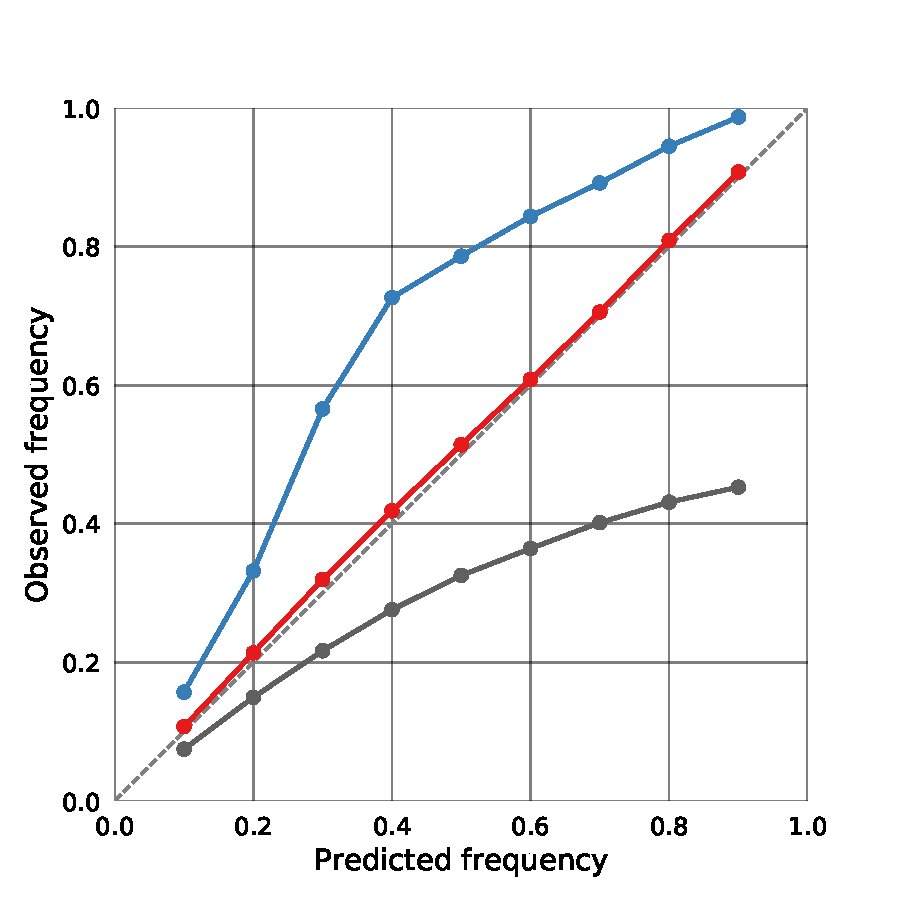
\includegraphics[width = 0.5\linewidth]{../plots/fig01}
  \caption{Example of a calibration plot displaying calibration curves for
           overly confident predictions (dark gray), well calibrated predictions (red),
           and overly cautious predictions (blue).}
  \label{fig:calibration_plot_example}
\end{figure}


%\section{Implementation}
%\label{sec:implementation}
%
%  In this section the implementation of the retrieval methods used in the
%  subsequent experiments is described. All three methods (MCMC, BCMI, QRNN) have
%  been implemented in Python \citep{python} and released as parts of the typhon
%  \citep{typhon} software package. The code for all calculations presented in
%  this paper is made available in the form of jupyter notebooks through public
%  repositories \citep{predictive_uncertainty, smhi}.
%
%\subsection{Markov Chain Monte Carlo}
%
%   The MCMC retrieval presented in Section~\ref{sec:synthetic} are based on
%   a Python implementation of the Metropolis algorithm \citep[Ch. 12]{bda}.
%   The implementation is designed to use the ARTS amtospheric radiative
%   transfer simulator \citep{arts_1, arts_2} as forwad model and has been
%   integrated into the typhon package.
%
%   The MCMC retrieval computes the a posteriori distribution of the integrated
%   column water vapor from passive microwave observations. The state space in
%   which the retrieval is performed is given by the temperature and water vapor
%   profiles of a plane parallel atmsophere. Proposal states are generated from a
%   random walk using the a priori covariance matrix scaled by an adaptive factor
%   that aims to keep the acceptance rate close to the optimal $21\%$
%   \citep{bda}.
%
%   A single MCMC retrieval consists of 8 independent runs, that are started with
%   different random states sampled from the a priori distribution. Each run
%   starts with a warm-up phase followed by an adaptive phase during which the
%   scaling of the covariance matrix of the proposal distribution is adapted. This is
%   followed by a production phase during which 5000 samples of the a posteriori
%   distribution are generated. Of these 5000 only 250 are kept in order to decrease
%   the correlation between the samples. To ensure sufficient convergence of the
%   simulations, the scale reduction factor $\hat{R}$ and the effective number of
%   independent samples \citep[eqs. (11.12), (11.13)]{bda} are computed. The
%   retrieval is discarded if the values are not smaller than 1.1 and larger than
%   100, respectively.
%   
%\subsection{Bayesian Monte Carlo Integration}
%
%  Also the BMCI method has been implemented in python and integrated into the
%  typhon package. The implementation provides functionality to speed up
%  calculations by excluding entries that are guaranteed to have a smaller weight
%  than a given limit. For the experiments presented below this was not used
%  since computational performance was not considered critical. In addition to
%  retrieving the first two moments of the posterior distribution, the
%  implementation also provides functionality to retrieve the posterior CDF using
%  Equation (\ref{eq:cdf}). Approximate posterior quantiles are computed by
%  interpolating the inverse CDF at the desired quantile values. To compute the
%  CRPS score for a given retrieval, the trapezoidal rule is used to perform the
%  integral over the values $x_i$ in the retrieval database $\{\vec{y}_i,
%  x_i\}_{i = 1}^n$.
%
%\subsection{Quantile Regression Neural Networks}
%
%    The implementation of quantile regression neural networks that has been
%    developed is based on the Keras Python package for deep learning
%    \citep{keras}. In order to enable the training of neural networks to predict
%    quantiles, the quantile loss function $\mathcal{L}_\tau(x_\tau, x)$ has been
%    implemented as a Keras-compatible loss function. The function can be
%    initiated with a sequence of quantile fratctions $\tau_1, \ldots, \tau_k$
%    allowing the neural network to learn to predict the corresponding quantiles
%    $x_{\tau_1}, \ldots, x_{\tau_k}$.
%
%    In addition to that, customized data generators have been added to the
%    implementation in order to allow the incorporation of information on
%    measurement uncertainty into the training process. If the training data is
%    noise free, the data generator can be used to add Gaussian noise to each
%    training batch according to the assumptions on measurement uncertainty. The
%    noise is added only directly before the data is passed to the neural network
%    keeping the original training data noise free. This ensures that the network
%    does not see the same, noisy training sample twice during training.
%
%    Here $\hat{\vec{x}}_\tau(\vec{y}_i)$ is the output predicted by the neural
%    network for the input $\vec{x}_i$. The batch presented to the network is
%    then simply given by the concatenation of the two batches.
%
%   For the training of the neural network an adaptive form of stochastic batch
%   gradient descent is used. During training, loss is monitored on a validation
%   set. When the loss on the validation set hasn't decreased for a certain number
%   of epochs, the training rate is reduced by a given reduction factor. The
%   training is stopped when a predefined minimum learning rate is reached.
%
%   The reconstruction of the CDF from the estimated quantiles is obtained
%   by using the quantiles as nodes of a piece-wise linear approximation and
%   extending the first and last segements out to 0 and 1, respectively.
%   This approximation is also used to compute the CRPS score on the test
%   data.



\section{Application to a synthetic retrieval case}
\label{sec:synthetic}

In this section, a simulated retrieval of column water vapor from passive
microwave observations is used to benchmark the performance of BMCI and QRNN
against MCMC simulation. The retrieval case has been set up to provide an
idealized but realistic scenario in which the true a posteriori distribution can
be approximated using MCMC simulation. The MCMC results can therefore be used as
the reference to investigate the retrieval performance of QRNNs and BMCI. Furthermore
it is investigated how different hyperparameters influence the performance of
the QRNN, and lastly how the size of the training set and retrieval database
impact the performance of QRNNs and BMCI.

\subsection{The retrieval}

   For this experiment, the retrieval of column water vapor (CWV) from passive
   microwave observations over the ocean is considered. The state of the
   atmosphere is represented by profiles of temperature and water vapor
   concentrations on 15 pressure levels between $10^3$ and $10\:\unit{hPa}$. The
   variability of these quantities has been estimated based on ECMWF ERA
   Interim data \citep{era_interim} from the year 2016, restricted to latitudes
   between $23^\circ$ and $66^\circ$ N. Parametrizations of the multivariate
   distributions of temperature and water vapor were obtained by fitting a joint
   multivariate normal distribution to the temperature and the logarithm of
   water vapor concentrations. The fitted distribution represents the a priori
   knowledge on which the simulations are based.

\subsubsection{Forward model simulations}

   The Atmospheric Radiative Transfer Simulator (ARTS, \citet{arts}) is used to
   simulate satellite observations of the atmospheric states sampled from the a
   priori distribution. The observations consist of simulated brightness
   temperatures from five channels around $23, 88, 165, 183 \unit{GHz}$
   (c.f. Table \ref{tab:channels}) of the ATMS sensor.

\begin{table}[hbpt]
\centering
\begin{tabular}{|r|c|c|c|}
    \hline
    Channel & Center frequency & Offset           & Bandwidth                \\ 
    \hline
                  1 & $23.8 \unit{GHz}$ &        ---       & $270 \unit{MHz}$ \\
                  2 & $88.2 \unit{GHz}$ &        ---       & $500 \unit{MHz}$ \\
                  3 & $165.5\unit{GHz}$ &        ---       & $300 \unit{MHz}$ \\
                  4 & $183.3\unit{GHz}$ & $7   \unit{GHz}$ & $2000\unit{MHz}$ \\
                  5 & $183.3\unit{GHz}$ & $3   \unit{GHz}$ & $1000\unit{MHz}$ \\
    \hline
\end{tabular}
\caption{Observation channels used for the synthetic retrieval of column water vapor.}
\label{tab:channels}
\end{table}

The simulations take into account only absorption and emission from water vapor.
Ocean surface emissivities are computed using the FASTEM-6 model \citep{fastem6}
with an assumed surface wind speed of zero. The sea surface temperature is
assumed to be equal to the temperature at the pressure level closest to the
surface but no lower than $270\unit{K}$. Sensor characteristics and absorption
lines are taken from the ATMS sensor descriptions that are provided within the
ARTS XML Data package. Simulations are performed for a nadir looking sensor and
neglecting polarization. The observation uncertainty is assumed to be
independent Gaussian noise with a standard deviation of $1\:\unit{K}$.


\subsubsection{MCMC implementation}

  The MCMC retrieval is based on a Python implementation of the Metropolis
  algorithm \citep[Ch. 12]{bda} that has been developed within the context of
  this study. It is released as part of the \textit{typhon: tools for atmospheric
  research} software package \citep{typhon}.

  The MCMC retrieval is performed in the space of atmospheric states described
  by the profiles of temperature and the logarithm of water vapor
  concentrations. The multivariate Gaussian distribution that has been obtained
  by fit to the ERA Interim data is taken as the a priori distribution. A random
  walk is used as the proposal distribution, with its covariance matrix taken as
  the a priori covariance matrix. A single MCMC retrieval consists of 8
  independent runs, initialized with different random states sampled from the a
  priori distribution. Each run starts with a warm-up phase followed by an
  adaptive phase during which the covariance matrix of the proposal distribution
  is scaled adaptively to keep the acceptance rate of proposed states close to
  the optimal $21\%$ \citep{bda}. This is followed by a production phase during
  which 5000 samples of the a posteriori distribution are generated. Only 1 out
  of 20 generated samples is kept in order to decrease the correlation between
  the resulting states. Convergence of each simulation is checked by computing
  the scale reduction factor $\hat{R}$ and the effective number of independent
  samples \citep[Eq. (11.12), (11.13)]{bda}. The retrieval is discarded if the
  values are not smaller than 1.1 and larger than 100, respectively. Each MCMC
  retrieval generates a sequence of atmospheric states from which the column
  water vapor is obtained by integration of the water vapor concentration
  profile. The distribution of observed CWV values is then taken as the
  retrieved a posteriori distribution.

  
\subsubsection{QRNN implementation}
\label{sec:implementation_qrnn}

  The implementation of quantile regression neural networks is based on the
  Keras Python package for deep learning \citep{keras}. It is also released
  part of the typhon package.

  For the training of quantile regression neural networks, the quantile loss
  function $\mathcal{L}_\tau(x_\tau, x)$ has been implemented so that it can be
  used as a training loss function within the Keras framework. The function can
  be initialized with a sequence of quantile fractions $\tau_1, \ldots,
  \tau_k$ allowing the neural network to learn to predict the corresponding
  quantiles $x_{\tau_1}, \ldots, x_{\tau_k}$.

  Custom data generators have been added to the implementation  to incorporate
   information on measurement uncertainty into the training
  process. If the training data is noise free, the data generator can be used to
  add noise to each training batch according to the assumptions on measurement
  uncertainty. The noise is added immediately  before the data is passed to the
  neural network, keeping the original training data noise free. This ensures
  that the network does not see the same, noisy training sample twice during
  training, thus counteracting overfitting.

% For the case that no specific assumptions
%  on measurement uncertainty can be made, a data generator for adversarial
%  training using the fast gradient sign method has been implemented. In this
%  case the perturbation factor $\delta_{\text{adv}}$ becomes an additional
%  hyperparameter of the network and needs to be tuned using independent
%  validation data. Since for this experiment the noise characteristics of the
%  sensor were known, this was not necessary here.

  An adaptive form of stochastic batch gradient descent is used for the neural
  network training. During the training, loss is monitored on a validation set.
  When the loss on the validation set hasn't decreased for a certain number of
  epochs, the training rate is reduced by a given reduction factor. The training
  stops when a predefined minimum learning rate is reached.

  The reconstruction of the CDF from the estimated quantiles is obtained
  by using the quantiles as nodes of a piece-wise linear approximation and
  extending the first and last segments out to 0 and 1, respectively.
  This approximation is also used to compute the CRPS score on the test
  data.


\subsubsection{BMCI implementation}
\label{sec:implementation_bmci}

 The BMCI method has likewise been implemented in Python and added to the
 typhon package. In addition to retrieving the first two moments of the
 posterior distribution, the implementation provides functionality to
 retrieve the posterior CDF using Eq.~(\ref{eq:bmci_cdf}). Approximate posterior
 quantiles are computed by interpolating the inverse CDF at the desired quantile
 values. To compute the CRPS score for a given retrieval, the trapezoidal rule
 is used to perform the integral over the values $x_i$ in the retrieval database
 $\{\vec{y}_i, x_i\}_{i = 1}^n$.

\subsection{QRNN model selection}

Just as with common neural networks, QRNNs have several hyperparameters that cannot
be learned directly from the data, but need to be tuned independently. For this
study the dependence of the QRNN performance on its hyperparameters has been
investigated. The results are included here as they may be a helpful reference
for future applications of QRNNs.

For this analysis, hyperparameters describing the structure of the QRNN model
are investigated separately from training parameters. The hyperparameters
describing the structure of the QRNN are:
\begin{enumerate}
  \item the number of hidden layers,
  \item the number of neurons per layer,
  \item the type of activation function.
  \setcounter{enumic}{\value{enumi}}
\end{enumerate}
The training method  described in Sect.~\ref{sec:implementation_qrnn} is
defined by the following training parameters:
\begin{enumerate}
  \setcounter{enumi}{\value{enumic}}
  \item the batch size used for stochastic batch gradient descent,
  \item the minimum learning rate at which the training is stopped,
  \item the learning rate decay factor,
  \item the number of training epochs without progress on the validation set
     before the learning rate is reduced.
\end{enumerate}

\subsubsection{Structural parameters}

  To investigate the influence of hyperparameters 1 - 3 on the performance of
  the QRNN, 10-fold cross validation on the training set consisting of $10^6$
  samples has been used to estimate the performance of different hyperparameter
  configurations. As performance metric the mean quantile loss on the validation
  set averaged over all predicted quantiles for $\tau = 0.05, 0.1, 0.2, \ldots, 0.9, 0.95$ 
  is used. A grid search over a subspace of the configuration space was
  performed to find optimal parameters. The results of the analysis are
  displayed in Figure~\ref{fig:hyperparams}. For the configurations considered,
  the layer width has the most significant effect on the performance.
  Nevertheless, only small performance gains are obtained by increasing the
  layer width to values above 64 neurons. Another general observation is that
  networks with three hidden layers generally outperform networks with fewer hidden
  layers. Networks using ReLU activation functions not only achieve slightly
  better performance than networks using tanh or sigmoid activation functions,
  but also show significantly lower variability. Based on these results, a
  neural network with three hidden layers, 128 neurons in each layer and ReLU
  activation functions has been selected for the comparison to BMCI.


  \begin{figure}[hbpt!]
    \centering
    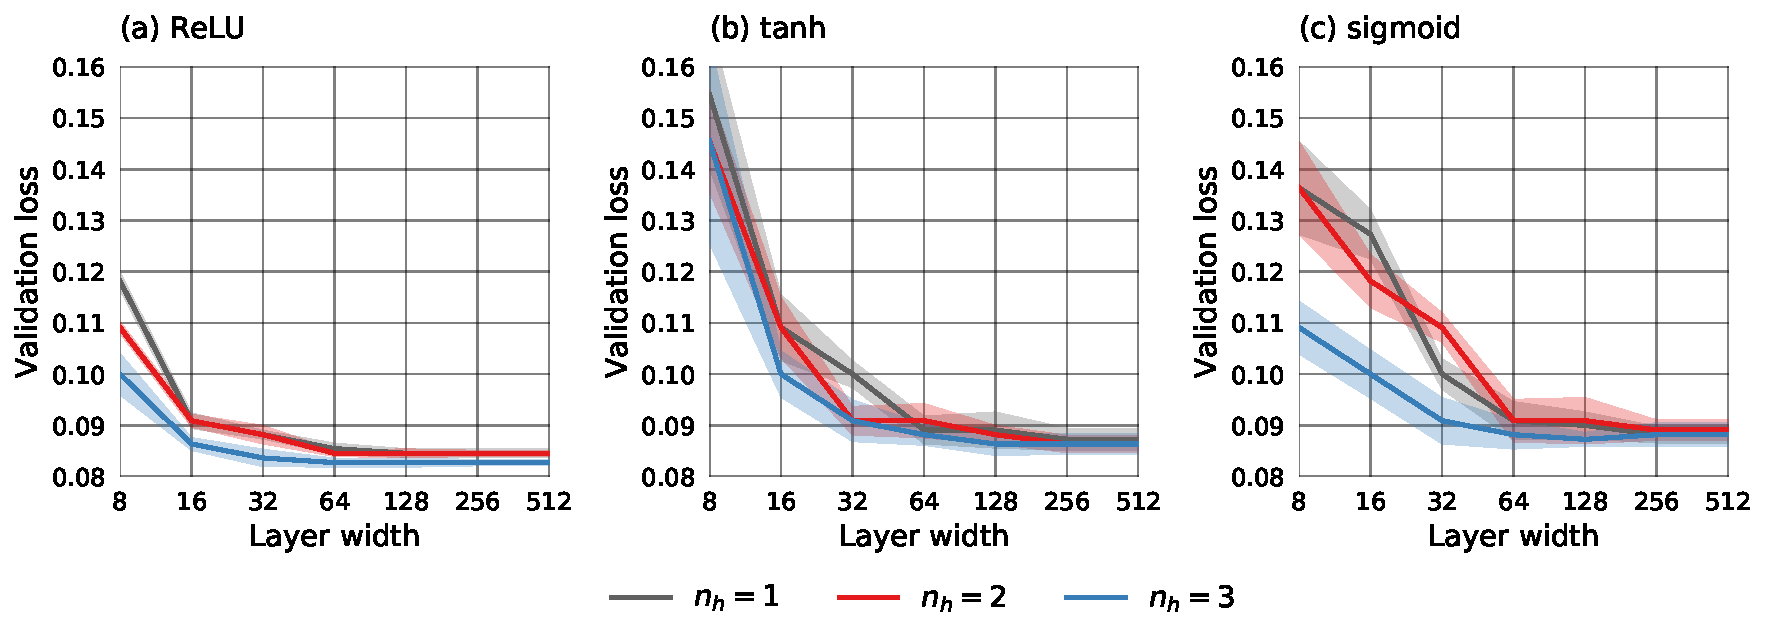
\includegraphics[width = 1.0\linewidth]{../plots/fig02}
    \caption{Mean validation set loss (solid lines) and standard deviation (shading)
             of different hyperparameter configurations with respect to layer width (number of neurons).
             Different lines display the results for different numbers of hidden layers $n_h$.
             The three panels show the results for ReLU, tanh, and sigmoid activation functions.}
    \label{fig:hyperparams}
  \end{figure}

 \subsubsection{Training parameters}
 
For the optimization of the training parameters 4 - 7, a very coarse grid
search was performed, using only three different values for each parameter.
In general, the training parameters showed only little effect ($< 2\%$ for the
combinations considered here) on the QRNN performance compared to the structural
parameters. The best cross-correlation performance was obtained for slow
training with a small learning rate reduction factor of $1.5$ and decreasing the
learning rate only after $10$ training epochs without reduction of the
validation loss. No significant increase in performance could be observed for
values of the learning rate minimum below $10^{-4}$. With respect to the batch
size, the best results were obtained for a batch size of 128 samples.
%However,
%while this very slow training works well for this example, a likely reason for
%this is the size and statistical homogeneity of the training and validation
%data. For real world data, a configuration that stops the training earlier 
%may yield better results.

\subsection{Comparison against MCMC}
  
%  The main purpose of the retrieval simulations is to provide a validation
%  and benchmark case for QRNNs. They were set up so that MCMC simulations
%  can be used to approximate the true a posteriori distribution. In this way,
%  the probabilistic predictions obtained from QRNNs (and BMCI) can be directly
%  compared to the approximated true a posteriori distribution.
  In this section, the performance of a single QRNN and an ensemble of 10 QRNNs
  are analyzed. The predictions from the ensemble are obtained by averaging the
  predictions from each network in the ensemble. All tests in this subsection are
  performed for a single QRNN, the ensemble of QRNNs, and BMCI. The retrieval database used
  for BMCI and the training of the QRNNs in this expirement consists of $10^6$ entries.

    Figure~\ref{fig:cdfs} displays retrieval results for eight example cases. The
choice of the cases is based on the Kolmogorov-Smirnov (KS) statistic, which
corresponds to the maximum absolute deviation of the predicted CDF from the
reference CDF obtained by MCMC simulation. A small KS value indicates a good
prediction of the true CDF, while a high value is obtained for large deviations
between predicted and reference CDF. The cases shown correspond to the 10th, 50th,
 90th and 99th percentile of the distribution of KS values obtained using BMCI
or a single QRNN. In this way they provide a qualitative overview of the performance
of the methods.

In the displayed cases, both methods are generally successful in predicting the
a posteriori distribution. Only for the $99$th percentile of the KS value distribution
does the BMCI prediction show significant deviations from the reference distribution.
 The jumps in the estimated a posteriori CDF indicate that the deviations are due to
undersampling of the input space in the retrieval database. This results in
overproportionally high weights attributed to the few entries close to the
observation. For this specific case the QRNN provides a better estimate of the a
posteriori CDF even though both predictions are based on the same data.

  \begin{figure}[hbpt!]
    \centering
    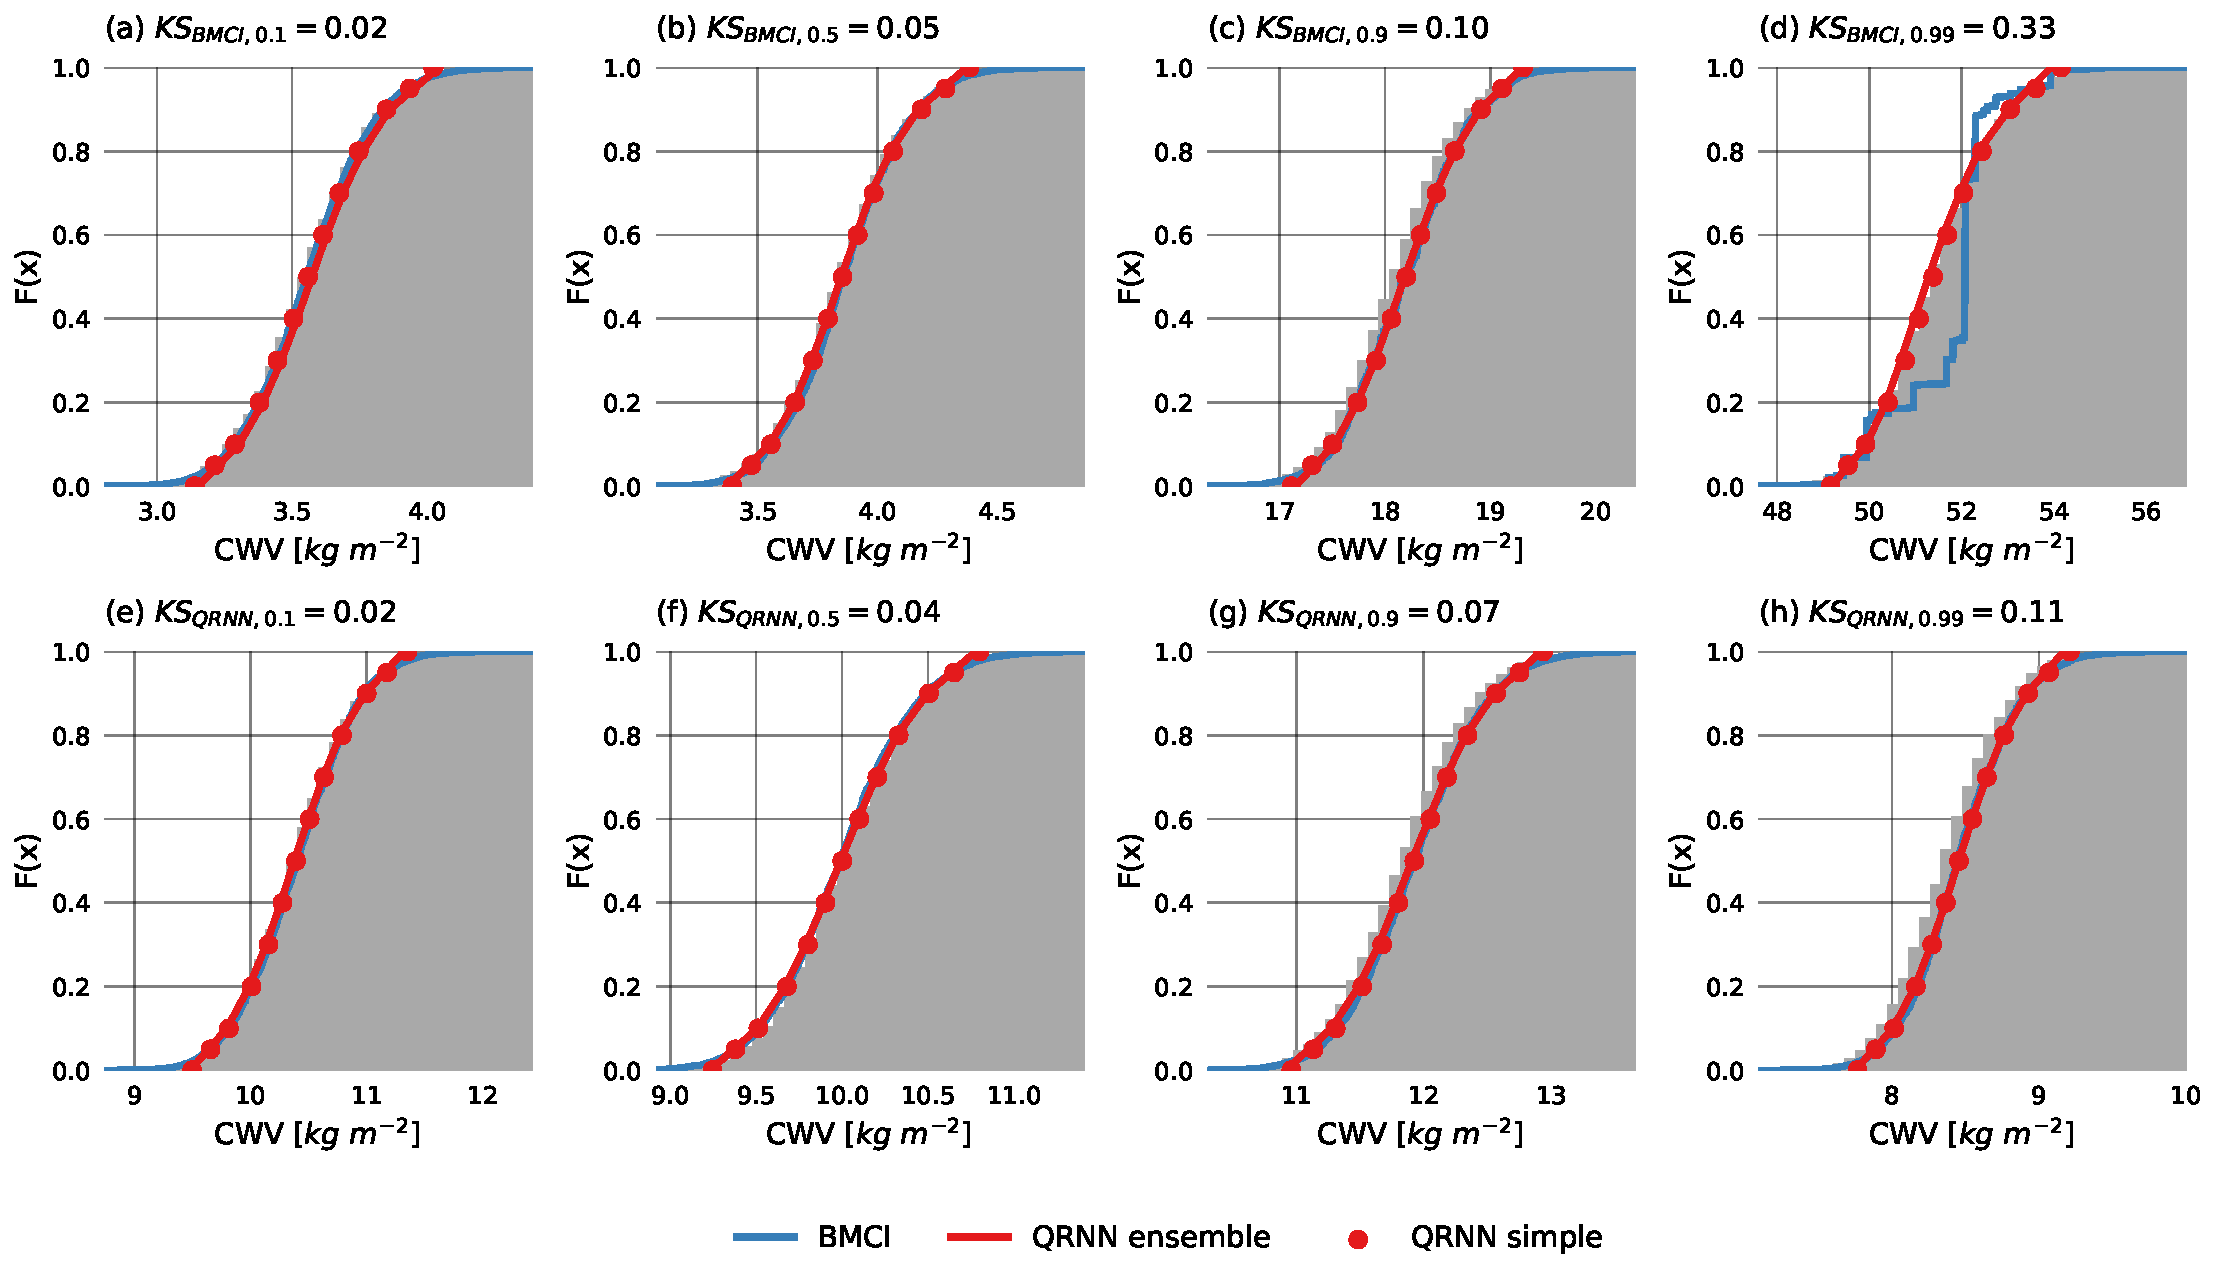
\includegraphics[width = 1.0\linewidth]{../plots/fig03}
    \caption{Retrieved a posteriori CDFs obtained using MCMC (grey), BMCI
    (blue), a single QRNN (red line) and an ensemble of QRNNs (red marker). Cases
    displayed in the first row correspond to the 1st, 50th, 90th, and 99th
    percentiles of the distribution of the Kolmogorov-Smirnov statistic of BMCI
    compared to the MCMC reference. The second row displays the same percentiles of
    the distribution of the Kolmogorov-Smirnov statistic of the single QRNN
    predictions compared to MCMC.}
    \label{fig:cdfs}
  \end{figure}

  To obtain a more comprehensive view on the performance of QRNNs and BMCI,
  the predictions obtained from both methods are compared to those obtained
  from MCMC for 6500 test cases. For the comparison, let the \textit{effective
    quantile fraction} $\tau_{\text{eff}}$ be defined as the fraction of MCMC
  samples that are less than or equal to the predicted quantile
  $\widehat{x_\tau}$ obtained from QRNN or BMCI. In general, the predicted
  quantile $\widehat{x_\tau}$ will not correspond exactly to the true quantile
  $x_\tau$, but rather an effective quantile $x_{\tau_\text{eff}}$, defined by
  the fraction $\tau_\text{eff}$ of the samples of the distribution that are
  smaller than or equal to the predicted value $\widehat{x_\tau}$. The
  resulting distributions of the effective quantile fractions for BMCI and
  QRNNs are displayed in Figure~\ref{fig:quantile_fractions} for the estimated
  quantiles for $\tau = 0.1, 0.2, \ldots, 0.9$.

  \begin{figure}[hbpt!]
    \centering
    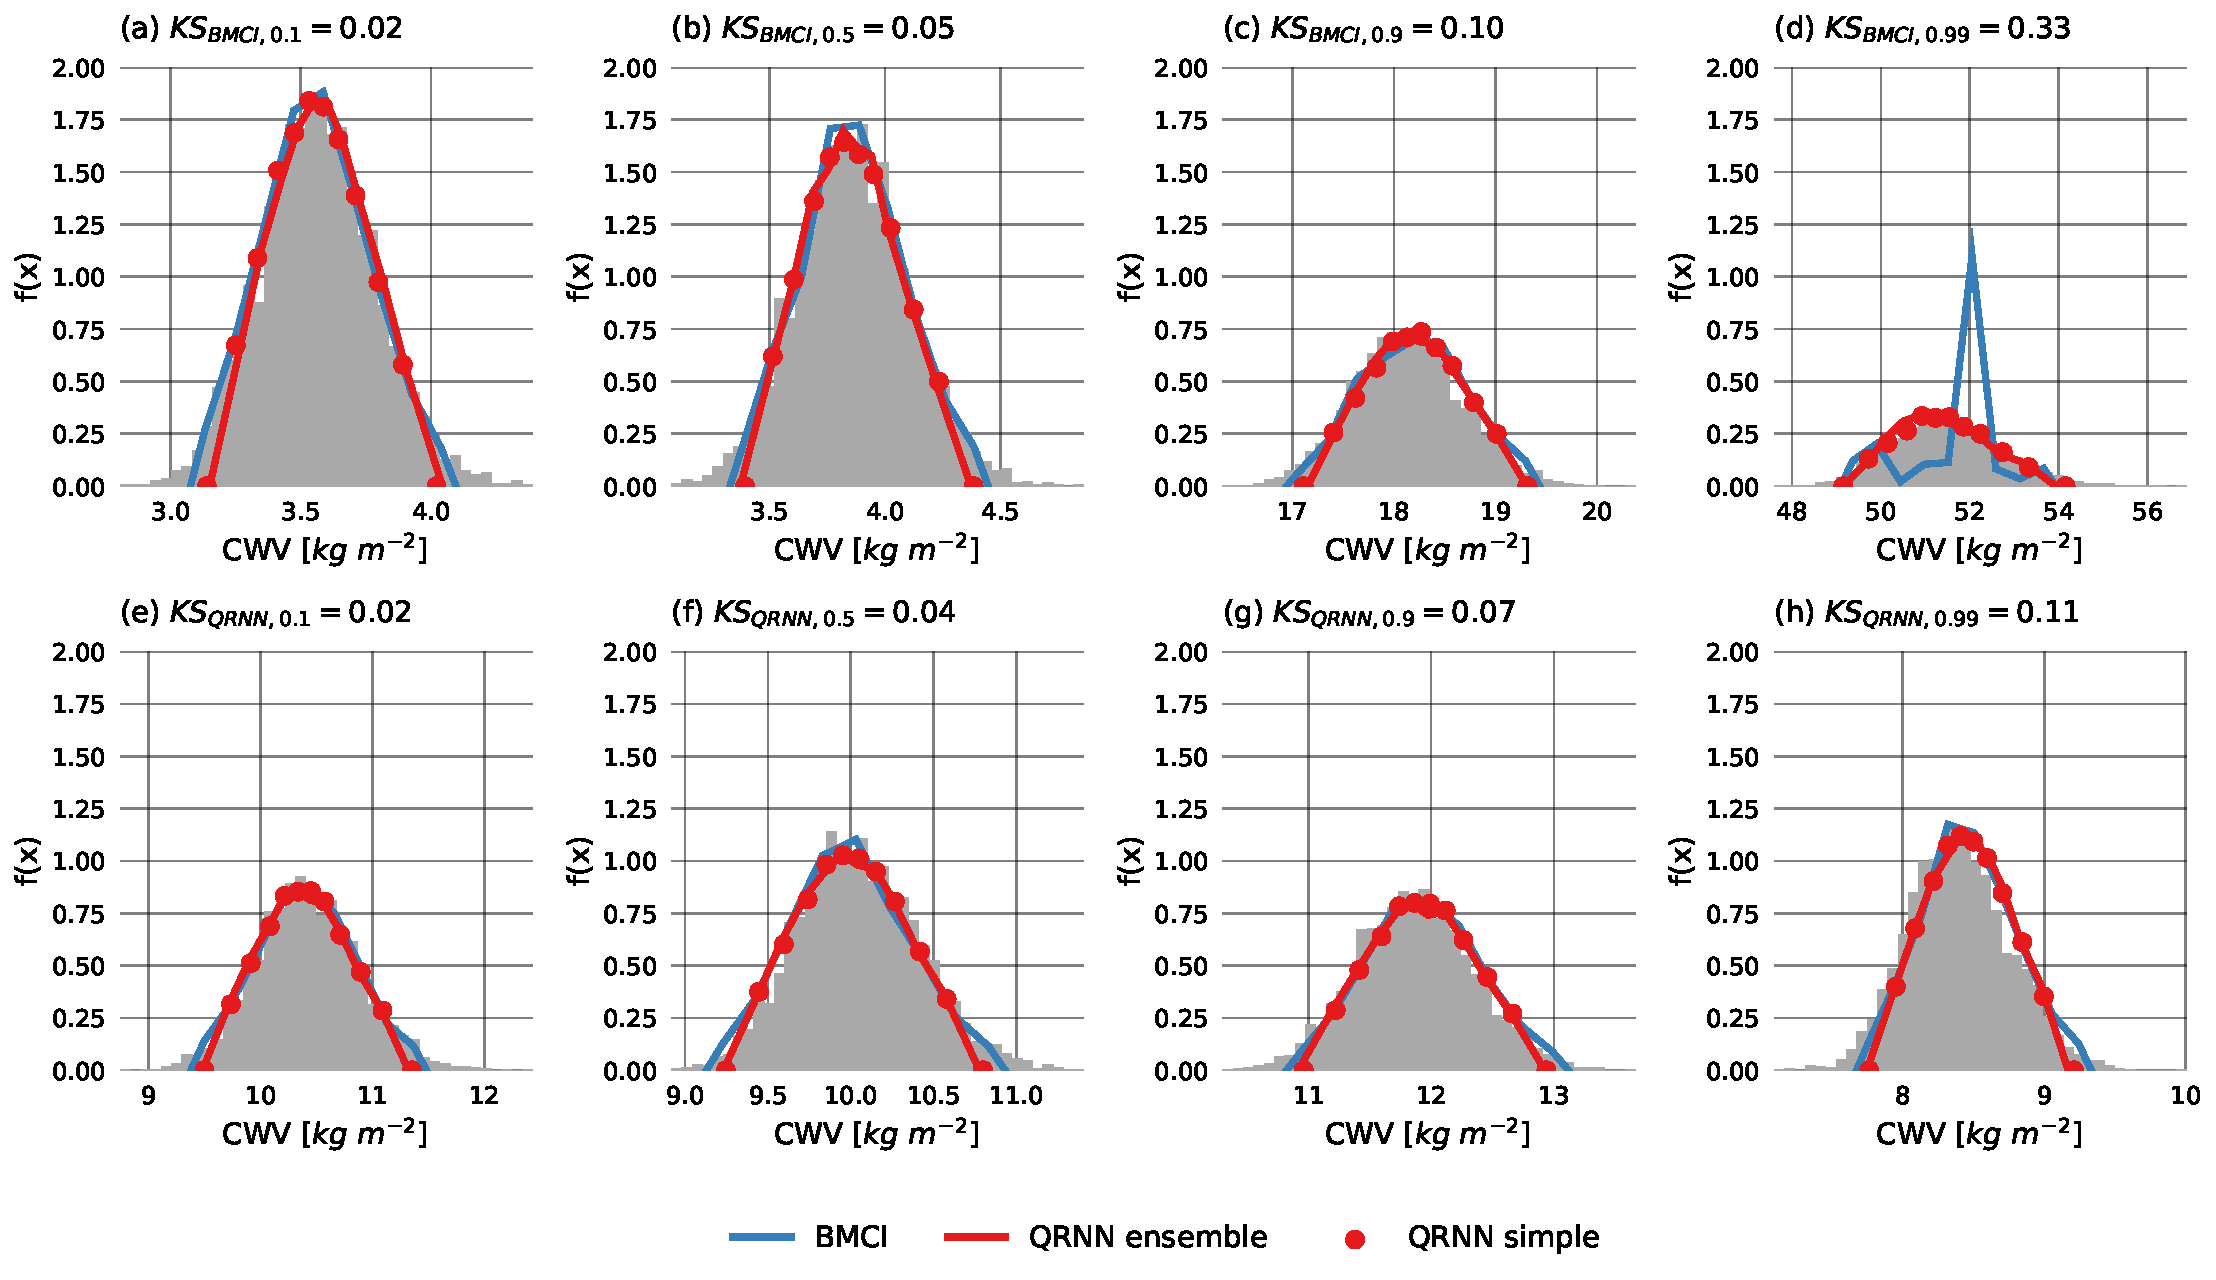
\includegraphics[width = 0.8\linewidth]{../plots/fig04}
    \caption{Distribution of effective quantile fractions $\tau_\text{eff}$ achieved by
      QRNN and BMCI on the test data. The left plot displays the performance of a
      single QRNN compared to BMCI, the right plot the performance of the ensemble.}
    \label{fig:quantile_fractions}
  \end{figure}

  For an ideal estimator of the quantile $x_\tau$, the resulting distribution
  would be a delta function centered at $\tau$. Due to the estimation error,
  however, the $\tau_{\text{eff}}$ values are distributed around the true quantile
  fraction $\tau$. The results show that both BMCI and QRNN provide fairly
  accurate estimates of the quantiles of the a posterior distribution. Furthermore,
  all methods  yield equally good predictions, making the distributions virtually
  identical.

\subsection{Training set size impact}

Finally, we investigate how the size of the training data set used in the training
of the QRNN (or as retrieval database for BMCI) affects the performance of the
retrieval method. This has been done by randomly generating training subsets
from the original training data with sizes logarithmically spaced between $10^3$
and $10^6$ samples. For each size, five random training subsets have been
generated and used to retrieve the test data with a single QRNN and BMCI. As test data,
a separate test set consisting of $10^5$ simulated observations vectors and
corresponding CWV values is used.

Figure~\ref{fig:mape_crps} displays the means of the mean absolute percentage
error (MAPE, Panel (a)) and the mean continuous ranked probability score (CRPS,
Panel (b)) achieved by both methods on the differently sized training sets.
For the computation of the MAPE, the CWV prediction is taken as the median of
the estimated a posteriori distribution obtained using QRNNs or BMCI. This value
is compared to the true CWV value corresponding to the atmospheric state that
has been used in the simulation. As expected, the performance of both methods
improves with the size of the training set. With respect to the MAPE, both
methods perform equally well for a training set size of $10^6$, but the QRNN
outperforms BMCI for all smaller training set sizes. With respect to CRPS, a
similar behavior is observed. These are reassuring results, as they indicate
that not only the accuracy of the predictions (measured by the MAPE and CRPS) improves
as the amount of training data increases, but also their calibration (measured
 only by the CRPS).

  \begin{figure}[hbpt!]
%    \centering
    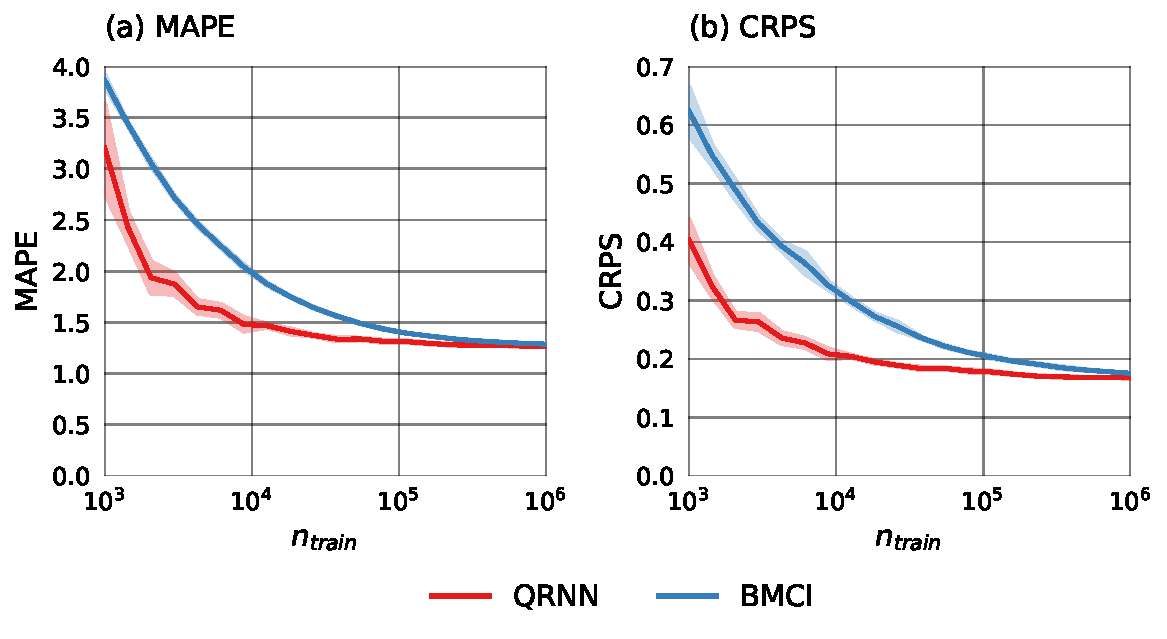
\includegraphics[width = 0.8\linewidth]{../plots/fig05}
    \caption{MAPE (Panel (a)) and CRPS (Panel (b)) achieved by QRNN (red) and BMCI (blue)
      on the test set using differently sized training sets and retrieval
    databases. For each size, five random subsets of the original training data were
    generated. The lines display the means of the observed values. The shading
    indicates the range of $\pm \sigma$ around the mean.}
    \label{fig:mape_crps}
  \end{figure}

Finally, the mean of the quantile loss $\mathcal{L}_\tau$ on the test set for
$\tau = 0.1, 0.5, 0.9$ has been considered (Figure~\ref{fig:quantile_losses}).
Qualitatively, the results are similar to the ones obtained using MAPE and CRPS.
The QRNN outperforms BMCI for smaller training set sizes but converges to similar
 values for training set sizes of $10^6$.

  \begin{figure}[hbpt!]
    \centering
    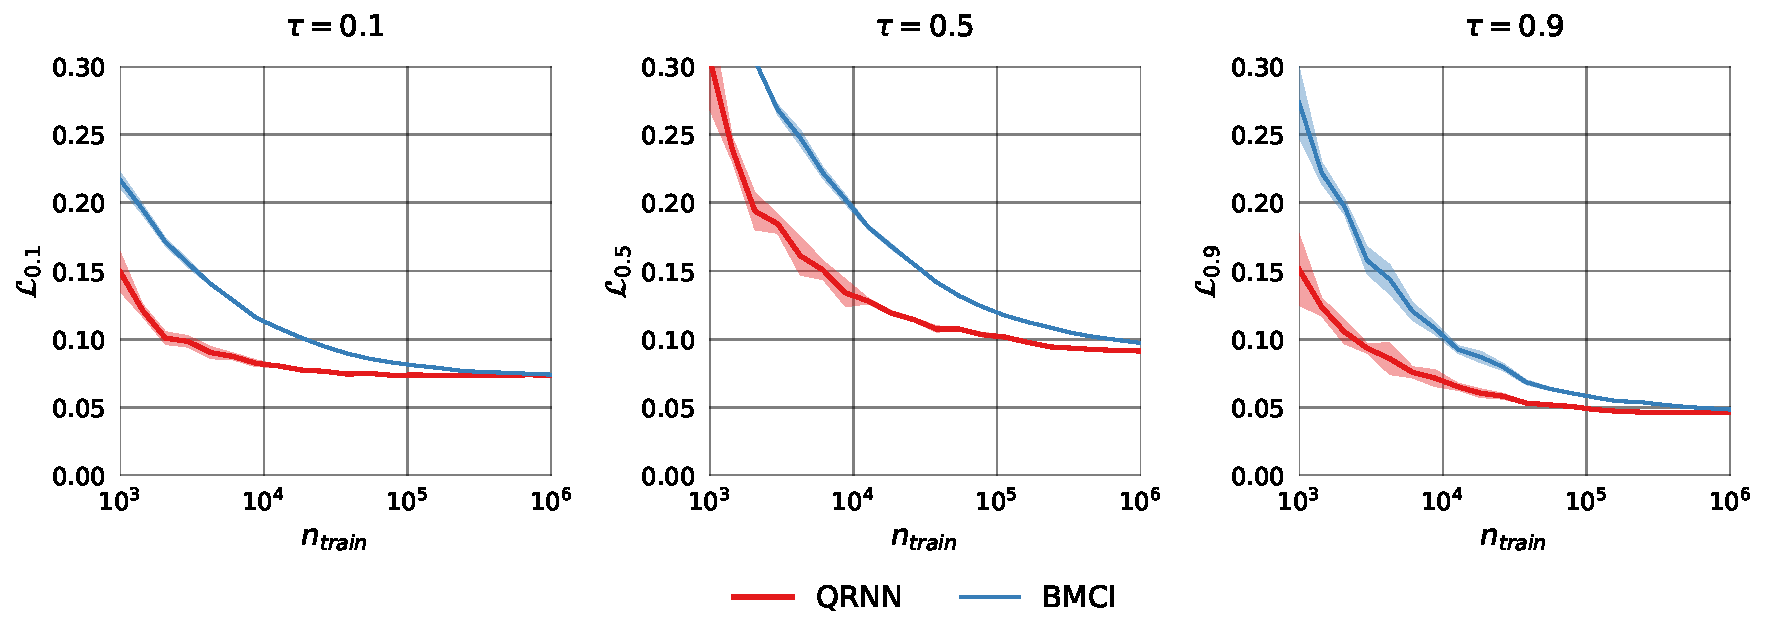
\includegraphics[width = 0.8\linewidth]{../plots/fig06}
    \caption{Mean quantile loss for different training set sizes $n_\text{train}$ and
    $\tau = 0.1, 0.5, 0.9$.}
    \label{fig:quantile_losses}
  \end{figure}

The results presented in this section indicate that QRNNs can, at least
under idealized conditions, be used to estimate the a posteriori distribution of 
Bayesian retrieval problems. Moreover, they were shown to work equally well
as BMCI for large data sets. What is interesting is that for smaller data sets,
QRNNs even provide better estimates of the a posteriori distribution than BMCI.
This indicates that QRNNs provide a better representation of the functional
dependency of the a posteriori distribution on the observation data, thus
achieving better interpolation in the case of scarce training data. Nonetheless,
 it remains to be investigated, if this advantage can also be observed for real
world data.

\section{Retrieving cloud top pressure from MODIS using QRNNs}
\label{sec:ctp}

In this section QRNNs are applied to retrieve cloud top pressure (CTP) using
observations from the moderate resolution imaging spectroradiometer (MODIS 
\citet{modis}). This experiment is based on the work by \cite{hakansson} who
developed a cloud top pressure retrieval algorithm (NN-CTTH) based on neural
networks. A QRNN based CTP retrieval is compared to the NN-CTTH algorithm and it
is investigated how QRNNs can be used to estimate the retrieval uncertainty.

\subsection{Data}

Exactly the same data as for the training of the NN-CTTH algorithm is used for
the training of the QRNNs. The data set consists of MODIS Level 1B data
\citep{myd021km, myd03} collocated with cloud properties obtained from CALIOP
\citep{calipso}. The \textit{top layer pressure} variable from the CALIOP data
is used as retrieval target. The data was taken from all orbits from 24 days
(the 1st and 14th of every month) from the year 2010. \citet{hakansson} train
neural networks using different combinations of input features and compare the
resulting performance. Only the $11 \unit{\mu m}$ and $12\unit{\mu m}$ channels
of MODIS are considered here, as they were found to yield a good compromise of
performance and flexibility. In addition to the single pixel input, structural
information is provided to the neural network in the form of various statistics
computed on a $5 \times 5$ neighborhood around the pixel. Furthermore, numerical
weather prediction data is provided to the network in the form of surface
pressure, temperatures at several pressure levels, and column integrated water
vapor.

The data used for the training of the QRNNs are the \textit{training} and
\textit{during-training validation set} from \cite{hakansson}. The QRNNs are
compared to the AVHRR version of the NN-CTTH algorithm, as this is the one
using the same input data for the retrieval. The comparison to NN-CTTH is
performed on the data set for \textit{testing under development}.

\subsection{Training}

The same training scheme as described in Sect.~\ref{sec:implementation_qrnn}
is used for the training of the QRNNs. The \textit{during-training validation} set is used
to monitor training progress based on which the learning rate is reduced or the
training stopped. After performing a grid search (results not shown) over width,
depth and minibatch size, the best performance on the validation set was
obtained for networks with four layers with 64 neurons each, ReLU activation functions,
 and a batch size of 128 samples.

The main difference in the training process compared to the previous experiment
is how measurement uncertainties are incorporated. For the simulated retrieval,
the training data was noise-free, so measurement uncertainties could be
realistically represented by adding noise according to the sensor
characteristics. This is not the case for MODIS observations; instead,
adversarial training is used here to ensure well-calibrated predictions. For the
tuning of the perturbation parameter $\delta_{\text{adv}}$ (c.f.
Sect.~\ref{sec:adversarial_training}), the calibration on the during-training
validation set was monitored using a calibration plot. Ideally, it would be
desirable to use a separate data set to tune this parameter, but this was
sufficient in this case to achieve good results on the test data. The calibration curves
obtained using different values of $\delta_\text{adv}$ are displayed in
Figure~\ref{fig:validation_calibration}. It can be seen from the plot that
without adversarial training ($\delta_\text{adv} = 0$) the predictions obtained
from the QRNN are overly confident, leading to prediction intervals that
underrepresent the uncertainty in the retrieval. Since adversarial training may
be viewed as a way of representing observation uncertainty in the training data,
larger values of $\delta_\text{adv}$ lead to less confident predictions. Based
on these results, $\delta_\text{adv} = 0.05$ is chosen for the training.

  \begin{figure}[hbpt!]
    \centering
    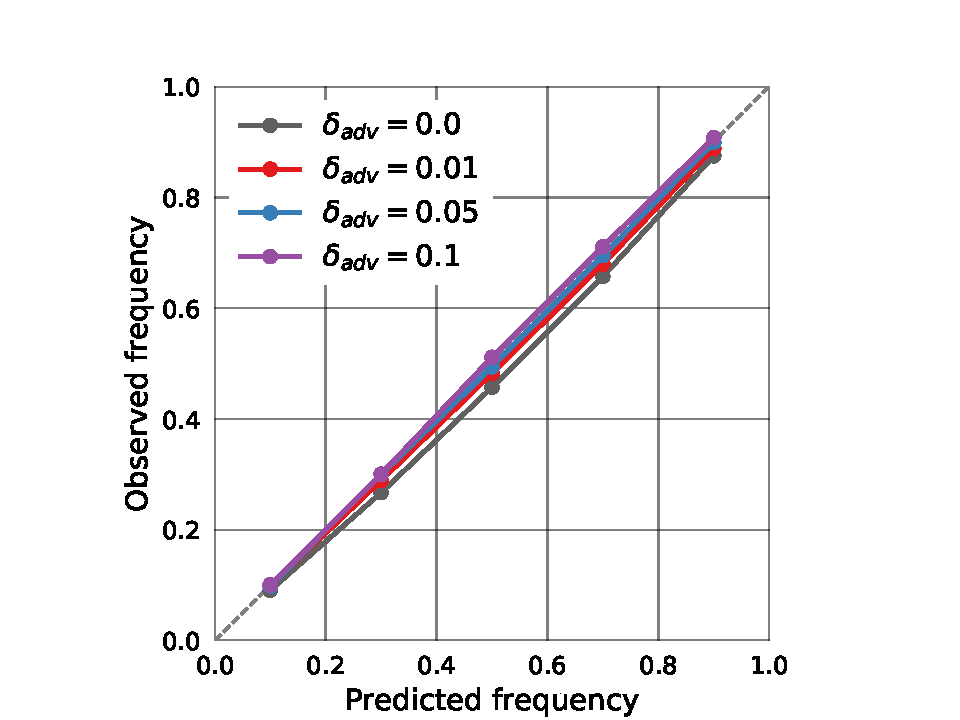
\includegraphics[width = 0.6\linewidth]{../plots/fig07}
    \caption{Calibration of the QRNN prediction intervals on the validation set
      used during training. The curves display the results for no adversarial training
      ($\delta_\text{adv} = 0$) and adversarial training with perturbation
      factor $\delta_\text{adv} = 0.01, 0.05, 0.1$.}
    \label{fig:validation_calibration}
  \end{figure}
  
Except for the use of adversarial training, the structure of the underlying
network and the training process of the QRNN are fairly similar to what is used
for the NN-CTTH retrieval. The QRNN uses four instead of two hidden layers with
64 neurons in each of them instead of 30 in the first and 15 in second layer.
While this makes the neural network used in the QRNN slightly more complex, this
should not be a major drawback since computational performance is generally not
critical for neural network retrievals.

\subsection{Prediction accuracy}


Figure~\ref{fig:ctp_results} displays the error distributions of the predicted
CTP values on the \textit{testing during development} data set. The error is
plotted separately for low, medium and high clouds (as classified by the CALIOP
feature classification flag) as well as the complete data set. For the QRNNs, the
prediction is taken as the median of the a posteriori distribution. Both the simple
QRNN and the ensemble of QRNNs perform slightly better than the NN-CTTH
algorithm for low and high clouds. For medium clouds, no significant difference
in the performance of the methods can be observed. The ensemble of QRNNs seems
to slightly improve upon the prediction accuracy of a single QRNN but the
difference is likely negligible.

\begin{figure}[hbpt!]
  \centering
  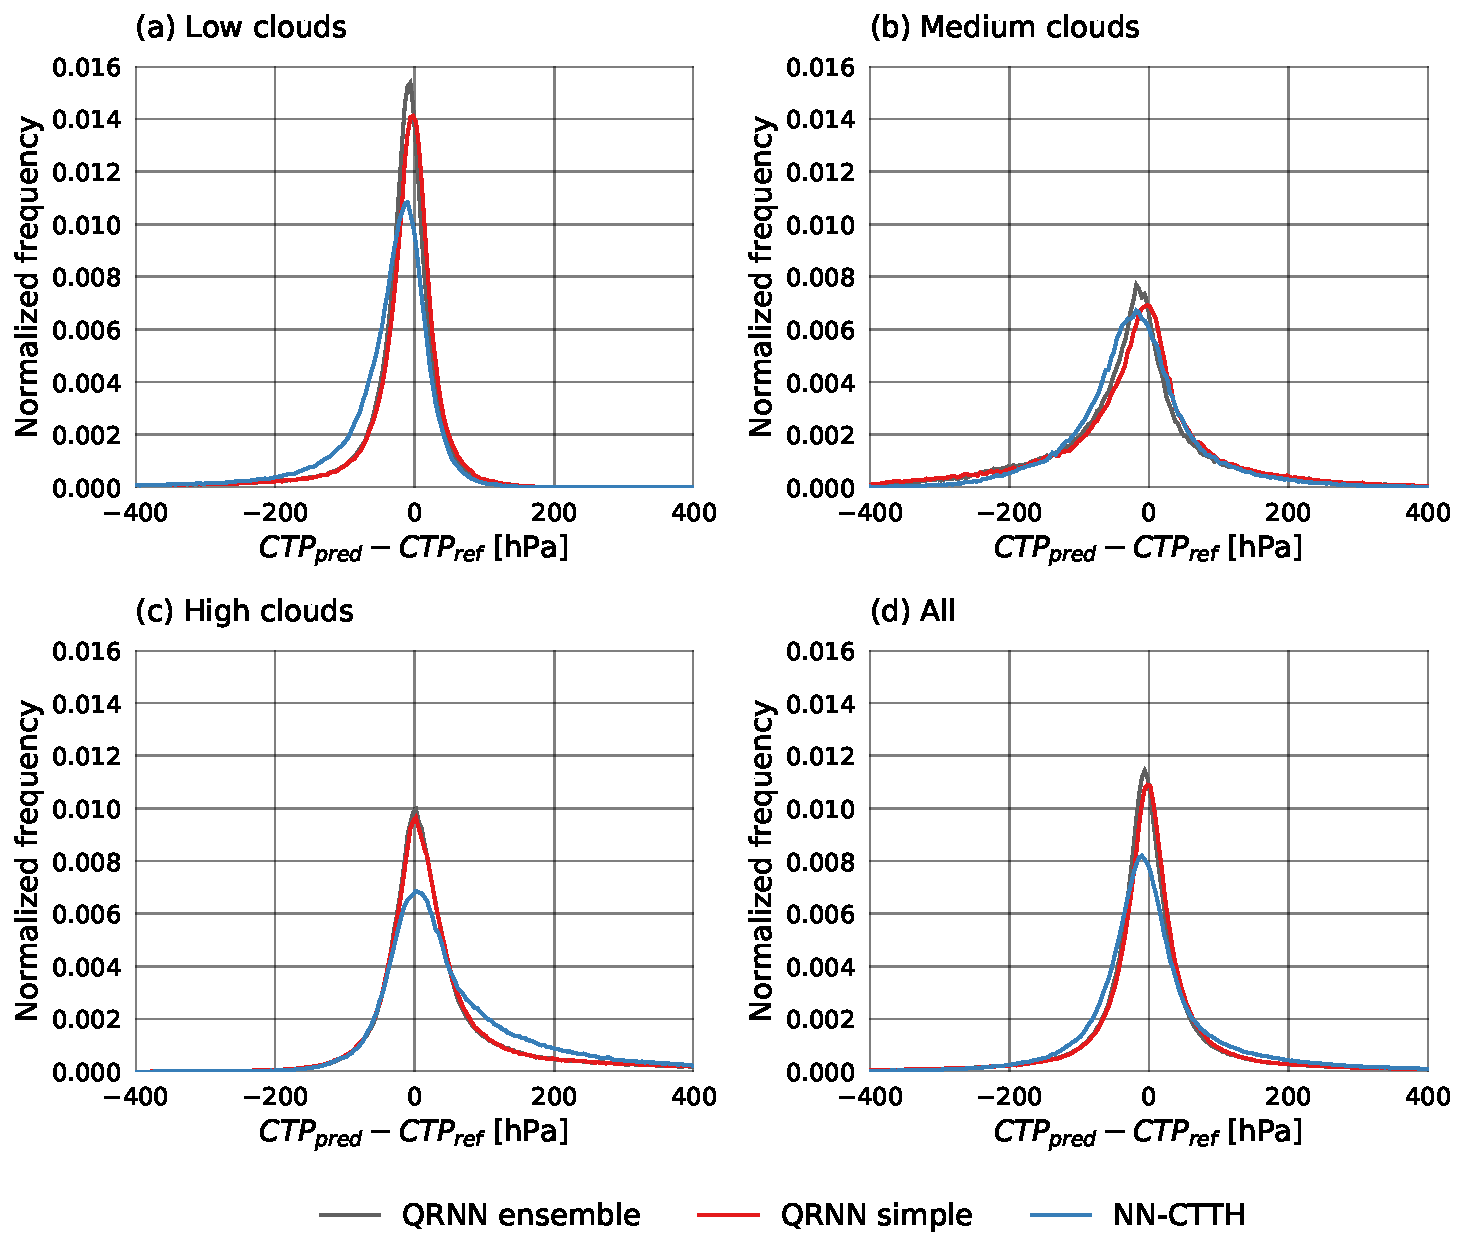
\includegraphics[width = 1.0\linewidth]{../plots/fig08}
  \caption{Error distributions of predicted CTP values $(\text{CTP}_{\text{pred}})$ with
    respect to CTP from CALIOP ($\text{CTP}_{\text{ref}}$) for different cloud types and the complete test set.}
  \label{fig:ctp_results}
\end{figure}

\subsection{Uncertainty estimation}

The NN-CTTH algorithm retrieves CTP but does not provide case-specific
uncertainty estimates. Instead, an estimate of uncertainty is provided in the
form of the observed mean absolute error on the test set. In order to compare
these uncertainty estimates with those obtained using QRNNs, Gaussian error
distributions are fitted to the observed error based on the observed mean
absolute error (MAE) and mean squared error (MSE). A Gaussian error model
is chosen here as it is arguably the most common distribution used to represent
random errors.

A plot of the errors observed on the \textit{testing during development} data
set and the fitted Gaussian error distributions is displayed in Panel (a) of
Figure~\ref{fig:error_fit}. The fitted error curves correspond to the Gaussian
probability density functions with the same MAE and MSE as observed on the test
data. Panel (b) displays the observed error together with the predicted error
obtained from a single QRNN. The predicted error is computed as the deviation of
a random sample of the estimated a posteriori distribution from its median. The
fitted Gaussian error distributions clearly do not provide a good fit to the
observed error. On the other hand, the predicted errors obtained from the QRNN a
posteriori distributions yield good agreement with the observed error. This
indicates that the QRNN successfully learned to predict retrieval uncertainties.
Furthermore, the results show that the ensemble of QRNNs actually provides a
slightly worse fit to the observed error than a single QRNN. An ensemble of
QRNNs thus does not necessarily improve the calibration of the predictions.

  \begin{figure}[hbpt!]
    \centering
    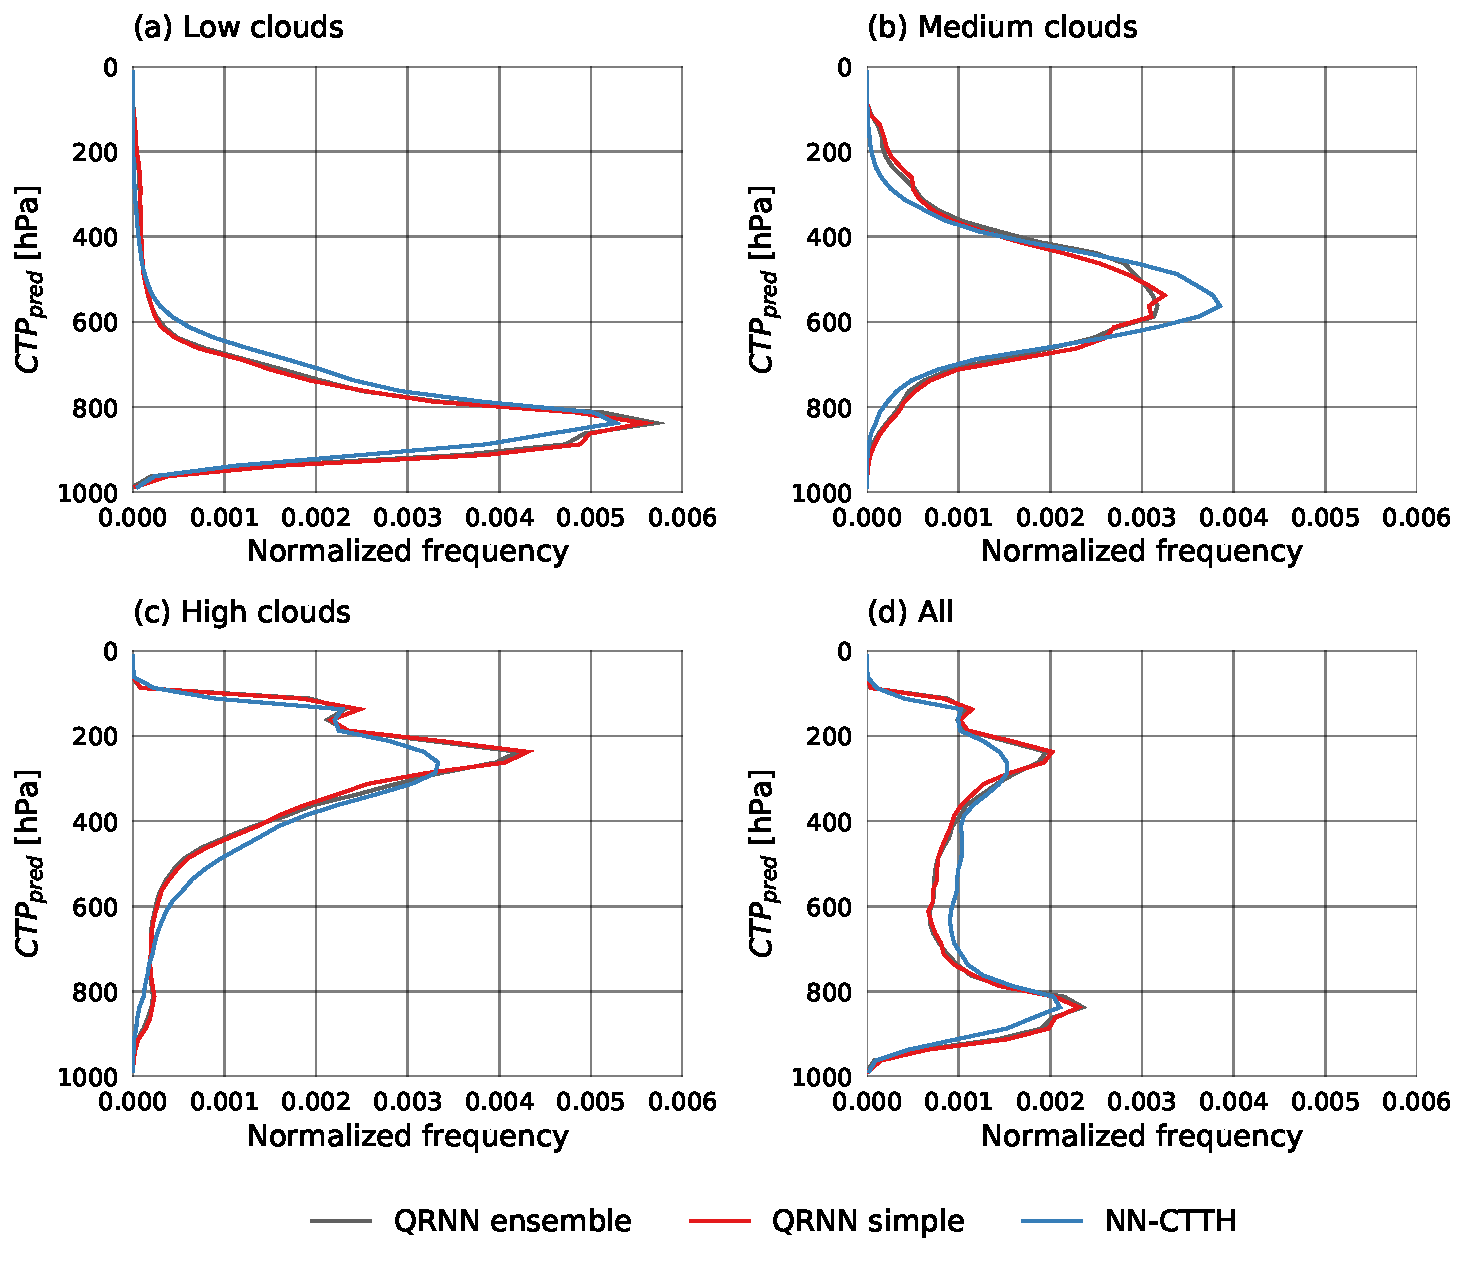
\includegraphics[width = 1.0\linewidth]{../plots/fig09.pdf}
    \caption{Predicted and observed error distributions. Panel (a)
      displays the observed error for the NN-CTTH retrieval as well as the
      Gaussian error distributions that have been fitted to the observed
      error distribution based on the MAE and MSE. Panel (b)
      displays the observed test set error for a single QRNN as well as the
      predicted error obtained as the deviation of a random sample of the
      predicted a posteriori distribution from the median. Panel (c) displays
      the same for the ensemble of QRNNs.}
    \label{fig:error_fit}
  \end{figure}

The Gaussian error model based on the MAE fit has also been used to produce
prediction intervals for the CTP values obtained from the NN-CTTH algorithm.
Figure~\ref{fig:calibration} displays the resulting calibration curves for the
NN-CTTH algorithm, a simple QRNN and an ensemble of QRNNs. The results support
the finding that a single QRNN is able to provide well calibrated probabilistic
predictions of the a posteriori distribution. The calibration curve for the
ensemble predictions is virtually identical to that for the single network. The
NN-CTTH predictions using a Gaussian fit are not as well calibrated and tend to
provide prediction intervals that are too wide for $p = 0.1, 0.3, 0.5, 0.7$ but
overly narrow intervals for $p = 0.9$.

  \begin{figure}[hbpt!]
    \centering
    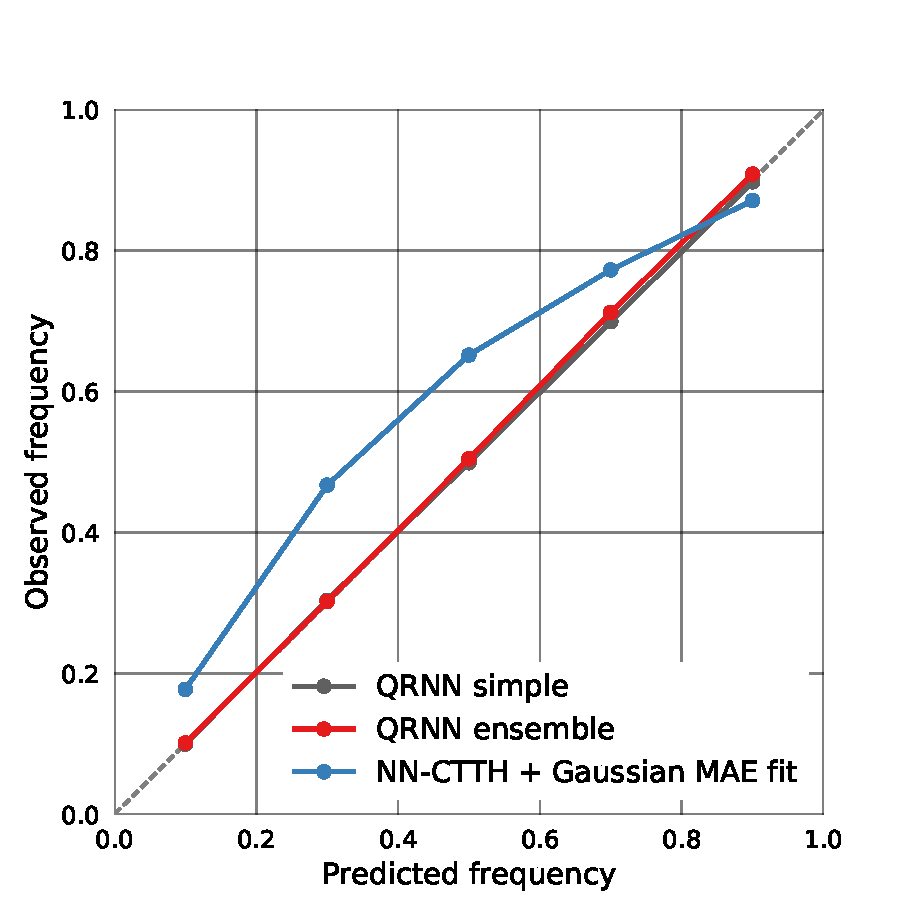
\includegraphics[width = 0.5\linewidth]{../plots/fig10}
    \caption{Calibration plot for prediction intervals derived from the Gaussian
      error model for the NN-CTTH algorithm (blue), the single QRNN (dark gray) and
      the ensemble of QRNNs (red).}
    \label{fig:calibration}
  \end{figure}

\subsection{Sensitivity to a priori distribution}

As shown above, the predictions obtained from the QRNN are statistically
consistent in the sense that they predict probabilities that match observed
frequencies when applied to test data. This however requires that the test data
is statistically consistent with the training data. Statistically consistent
here means that both data sets come from the same generating distribution, or in
more Bayesian terms, the same a priori distribution. What happens when this is
not the case can be seen when the calibration with respect to different cloud
types is computed. Figure~\ref{fig:calibration_cloud_type} displays calibration
curves computed separately for low, medium and high clouds. As can be seen from the plot, the QRNN
predictions are no longer equally well calibrated. Viewed from the Bayesian
perspective, this is not very surprising as CTP values for median clouds have a
significantly different a priori distribution compared to CTP values for all
cloud types, thus giving different a posteriori distributions.

 For the NN-CTTH algorithm, the results look different. While for low clouds
the calibration deteriorates, the calibration is even slightly improved for
high clouds. This is not surprising as the Gaussian fit may be more
appropriate on different subsets of the test data. 

  \begin{figure}[hbpt!]
    \centering
    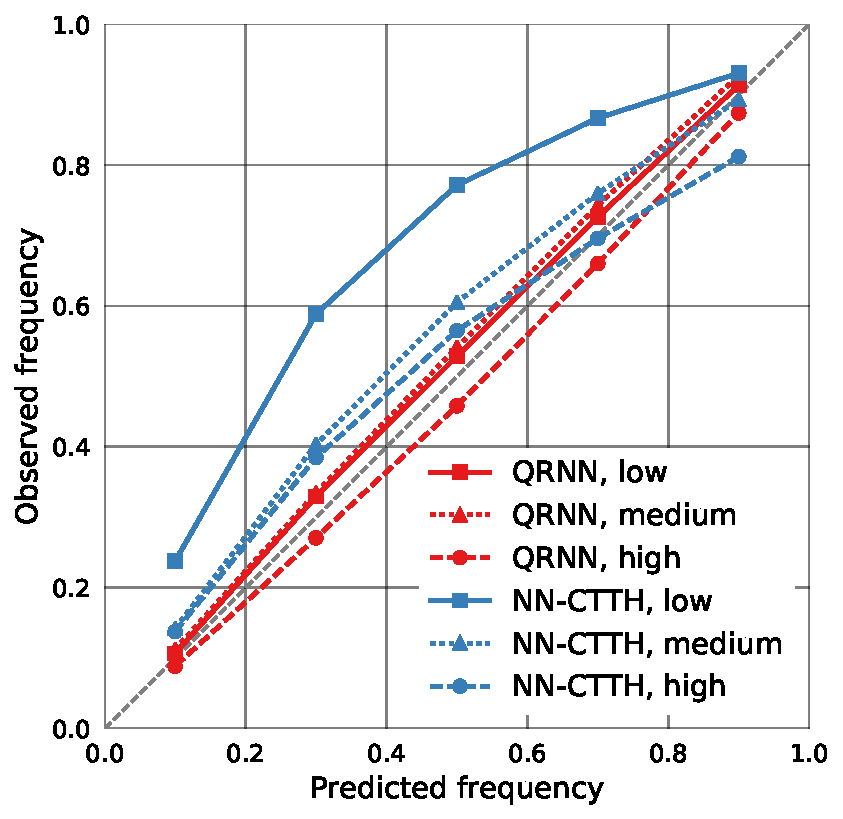
\includegraphics[width = 0.5\linewidth]{../plots/fig11}
    \caption{Calibration of the prediction intervals obtained from NN-CTTH (blue) and
      a single QRNN (red) with respect to specific cloud types.}
    \label{fig:calibration_cloud_type}
  \end{figure}


\conclusions  %% \conclusions[modified heading if necessary]
\label{sec:conclusions}

In this article, quantile regression neural networks have been proposed as a
method to estimate a posteriori distributions of Bayesian remote sensing retrievals.
They have been applied to two retrievals of scalar atmospheric variables. It has
been demonstrated that QRNNs are capable of providing accurate and
well-calibrated probabilistic predictions in agreement with the Bayesian
formulation of the retrieval problem.

The synthetic retrieval case presented in Sect.~\ref{sec:synthetic} shows that
the conditional distribution learned by the QRNN is the same as the Bayesian a
posteriori distribution obtained from methods that are directly based on the
Bayesian formulation. This in itself seems worthwhile to note, as it reveals the
importance of the training set statistics that implicitly represent the a priori
knowledge. On the synthetic data set, QRNNs compare well to BMCI and even perform
better for small data sets. This indicates that they are able to handle the
``curse of dimensionality'' \citep{friedman} better than BMCI, which would make them more suitable
for the application to retrieval problems with high-dimensional measurement
spaces.

While the optimization of computational performance of the BMCI method has not been
investigated in this work, at least compared to a naive implementation of BMCI,
QRNNs allow for at least one order of magnitude faster retrievals. QRNN retrievals
can be easily parallelized and hardware optimized implementations are available
for all modern computing architectures, thus providing very good performance out
of the box.

Based on these very promising results, the next step in this line of research
should be to compare QRNNs and BMCI on a real retrieval case to investigate if
the findings from the simulations carry over to the real world. If this is the
case, significant reductions in the computational cost of operational retrievals
and maybe even better retrieval performance could be achieved using QRNNs.

In the second retrieval application presented in this article, QRNNs have been
used to retrieve cloud top pressure from MODIS observations. The results show
that not only are QRNNs able to improve upon state-of-the-art retrieval accuracy
but they can also learn to predict retrieval uncertainty. The ability of QRNNs
to provide statistically consistent, case-specific uncertainty estimates should
make them a very interesting alternative to non-probabilistic neural network
retrievals. Nonetheless, also the sensitivity of the QRNN approach to a priori
assumptions has been demonstrated. The posterior distribution learned by the
QRNN depends on the validity of the a priori assumptions encoded in the training
data. In particular, accurate uncertainty estimates can only be expected if the
retrieved observations follow the same distribution as the training data. This,
however, is a limitation inherent to all empirical methods.

The second application case presented here demonstrated the ability of QRNNs to represent
non-Gaussian retrieval errors. While, as shown in this study, this is also the case
for BMCI (Eq.~(\ref{eq:bmci_cdf})), it is common in practice to estimate only mean and standard
deviation of the a posteriori distribution. Furthermore, implementations usually
assume Gaussian measurement errors, which is an unlikely assumption if the
observations in the retrieval database contain modeling errors. By requiring no
assumptions whatsoever on the involved uncertainties, QRNNs may provide a more
suitable way of representing (non-Gaussian) retrieval uncertainties.

The application of the Bayesian framework to neural network retrievals opens the
door to a number of interesting applications that could be pursued in future
research. It would for example be interesting to investigate if the a priori
information can be separated from the information contained in the retrieved
measurement. This would make it possible remove the dependency of the
probabilistic predictions on the a priori assumptions, which can currently be
considered a limitation of the approach. Furthermore, estimated a posteriori
distributions obtained from QRNNs could be used to estimate the information
content in a retrieval following the methods outlined by \citet{rodgers}.

In this study only the retrieval of scalar quantities was considered. Another
aspect of the application of QRNNs to remote sensing retrievals that remains to
be investigated is how they can be used to retrieve vector-valued retrieval
quantities. While the generalization to marginal, multivariate quantiles should
be straight forward, it is unclear whether a better approximation of the
quantile contours of the joint a posteriori distribution can be obtained using
QRNNs.

%What has not been considered in this work is the quantification of
%out-of-distribution uncertainty, which refers to uncertainty due to statistical
%differences between the training data and the data to which the neural network
%is applied. It has been shown by \citet{lakshminarayanan} that ensemble methods
%can be used to detect out-of-sample application of neural networks. It would
%therefore be interesting to investigate if and how ensembles of QRNN can be used
%to detect out-of-sample uncertainty.


%% The following commands are for the statements about the availability of data sets and/or software code corresponding to the manuscript.
%% It is strongly recommended to make use of these sections in case data sets and/or software code have been part of your research the article is based on.

\codeavailability{The implementation of the retrieval methods that were used in
this article have been published as parts of the \textit{typhon: tools for
atmospheric research} \citep{typhon} software package. The source code for the
calculations presented in Sect.~\ref{sec:synthetic} and \ref{sec:ctp} are
accessible from public repositories \citep{predictive_uncertainty, smhi}.}


%\dataavailability{TEXT} %% use this section when having only data sets available


%\codedataavailability{TEXT} %% use this section when having data sets and software code available





%\appendix
%\section{}    %% Appendix A
%
%\subsection{}     %% Appendix A1, A2, etc.


\noappendix       %% use this to mark the end of the appendix section

%% Regarding figures and tables in appendices, the following two options are possible depending on your general handling of figures and tables in the manuscript environment:

%% Option 1: If you sorted all figures and tables into the sections of the text, please also sort the appendix figures and appendix tables into the respective appendix sections.
%% They will be correctly named automatically.

%% Option 2: If you put all figures after the reference list, please insert appendix tables and figures after the normal tables and figures.
%% To rename them correctly to A1, A2, etc., please add the following commands in front of them:

%\appendixfigures  %% needs to be added in front of appendix figures
%
%\appendixtables   %% needs to be added in front of appendix tables
%
%  \begin{table}[ht]
%  \begin{center}
%
%    \vspace{0.5cm}
%    \resizebox{\textwidth}{!}{
%     \begin{tabular}{|l|ccccccc|}
%     \multicolumn{8}{c}{Linear}\\
%     \hline
%     \input{../tables/linear.tbl}
%     \end{tabular}}
%
%    \vspace{0.5cm}
%    \resizebox{\textwidth}{!}{
%     \begin{tabular}{|l|ccccccc|}
%     \multicolumn{8}{c}{Sigmoid}\\
%     \hline
%     \input{../tables/sigmoid.tbl}
%     \end{tabular}}
%
%    \vspace{0.5cm}
%    \resizebox{\textwidth}{!}{
%     \begin{tabular}{|l|ccccccc|}
%     \multicolumn{8}{c}{tanh}\\
%     \hline
%     \input{../tables/tanh.tbl}
%     \end{tabular}}
%
%    \vspace{0.5cm}
%    \resizebox{\textwidth}{!}{
%     \begin{tabular}{|l|ccccccc|}
%     \multicolumn{8}{c}{ReLU}\\
%     \hline
%     \input{../tables/relu.tbl}
%     \end{tabular}}
%
%    \caption{Mean quantile loss and standard deviation for different activation functions, varying numbers
%             $n_h$ of hidden layers and $n_n$ of neurons per layer. Results were obtained using 10-fold
%             cross validation on the training set.}
%
% \label{tab:model_selection}
%
%  \end{center}
% \end{table} 

%% Please add \clearpage between each table and/or figure. Further guidelines on figures and tables can be found below.



\authorcontribution{All authors contributed to the study through discussion and
feedback. Patrick Eriksson and Bengt Rydberg proposed the application of QRNNs
to remote sensing retrievals. The study was designed and implemented by Simon Pfreundschuh,
who also prepared the manuscript including figures, text and tables.
Anke Thoss and Nina H{\aa}kansson provided the training data for the cloud top
pressure retrieval.} %% optional section

\competinginterests{The authors declare that they have no conflict of interest.} %% this section is mandatory even if you declare that no competing interests are present

%\disclaimer{TEXT} %% optional section

\begin{acknowledgements}
The scientists at Chalmers University of Technology were funded by the Swedish National Space Board.

The authors would like to acknowledge the work of Ronald Scheirer and Sara
Hörnquist who were involved in the creation of the collocation dataset that was
used as training and test data for the cloud top pressure retrieval.

Numerous free software packages were used to perform the numerical experiments
presented in this article and visualize their results. The authors would like to
acknowledge the work of all the developers that contributed to making these tools
freely available to the scientific community, in particular the work by
\citet{matplotlib, ipython, numpy, python}.
\end{acknowledgements}




%% REFERENCES

%% The reference list is compiled as follows:


%% Since the Copernicus LaTeX package includes the BibTeX style file copernicus.bst,
%% authors experienced with BibTeX only have to include the following two lines:
%%
\bibliographystyle{copernicus}
\bibliography{literature.bib}
%%
%% URLs and DOIs can be entered in your BibTeX file as:
%%
%% URL = {http://www.xyz.org/~jones/idx_g.htm}
%% DOI = {10.5194/xyz}


%% LITERATURE CITATIONS
%%
%% command                        & example result
%% \citet{jones90}|               & Jones et al. (1990)
%% \citep{jones90}|               & (Jones et al., 1990)
%% \citep{jones90,jones93}|       & (Jones et al., 1990, 1993)
%% \citep[p.~32]{jones90}|        & (Jones et al., 1990, p.~32)
%% \citep[e.g.,][]{jones90}|      & (e.g., Jones et al., 1990)
%% \citep[e.g.,][p.~32]{jones90}| & (e.g., Jones et al., 1990, p.~32)
%% \citeauthor{jones90}|          & Jones et al.
%% \citeyear{jones90}|            & 1990



%% FIGURES

%% When figures and tables are placed at the end of the MS (article in one-column style), please add \clearpage
%% between bibliography and first table and/or figure as well as between each table and/or figure.


%% ONE-COLUMN FIGURES

%%f
%\begin{figure}[t]
%\includegraphics[width=8.3cm]{FILE NAME}
%\caption{TEXT}
%\end{figure}
%
%%% TWO-COLUMN FIGURES
%
%%f
%\begin{figure*}[t]
%\includegraphics[width=12cm]{FILE NAME}
%\caption{TEXT}
%\end{figure*}
%
%
%%% TABLES
%%%
%%% The different columns must be seperated with a & command and should
%%% end with \\ to identify the column brake.
%
%%% ONE-COLUMN TABLE
%
%%t
%\begin{table}[t]
%\caption{TEXT}
%\begin{tabular}{column = lcr}
%\tophline
%
%\middlehline
%
%\bottomhline
%\end{tabular}
%\belowtable{} % Table Footnotes
%\end{table}
%
%%% TWO-COLUMN TABLE
%
%%t
%\begin{table*}[t]
%\caption{TEXT}
%\begin{tabular}{column = lcr}
%\tophline
%
%\middlehline
%
%\bottomhline
%\end{tabular}
%\belowtable{} % Table Footnotes
%\end{table*}
%
%
%%% MATHEMATICAL EXPRESSIONS
%
%%% All papers typeset by Copernicus Publications follow the math typesetting regulations
%%% given by the IUPAC Green Book (IUPAC: Quantities, Units and Symbols in Physical Chemistry,
%%% 2nd Edn., Blackwell Science, available at: http://old.iupac.org/publications/books/gbook/green_book_2ed.pdf, 1993).
%%%
%%% Physical quantities/variables are typeset in italic font (t for time, T for Temperature)
%%% Indices which are not defined are typeset in italic font (x, y, z, a, b, c)
%%% Items/objects which are defined are typeset in roman font (Car A, Car B)
%%% Descriptions/specifications which are defined by itself are typeset in roman font (abs, rel, ref, tot, net, ice)
%%% Abbreviations from 2 letters are typeset in roman font (RH, LAI)
%%% Vectors are identified in bold italic font using \vec{x}
%%% Matrices are identified in bold roman font
%%% Multiplication signs are typeset using the LaTeX commands \times (for vector products, grids, and exponential notations) or \cdot
%%% The character * should not be applied as mutliplication sign
%
%
%%% EQUATIONS
%
%%% Single-row equation
%
%\begin{equation}
%
%\end{equation}
%
%%% Multiline equation
%
%\begin{align}
%& 3 + 5 = 8\\
%& 3 + 5 = 8\\
%& 3 + 5 = 8
%\end{align}
%
%
%%% MATRICES
%
%\begin{matrix}
%x & y & z\\
%x & y & z\\
%x & y & z\\
%\end{matrix}
%
%
%%% ALGORITHM
%
%\begin{algorithm}
%\caption{...}
%\label{a1}
%\begin{algorithmic}
%...
%\end{algorithmic}
%\end{algorithm}
%
%
%%% CHEMICAL FORMULAS AND REACTIONS
%
%%% For formulas embedded in the text, please use \chem{}
%
%%% The reaction environment creates labels including the letter R, i.e. (R1), (R2), etc.
%
%\begin{reaction}
%%% \rightarrow should be used for normal (one-way) chemical reactions
%%% \rightleftharpoons should be used for equilibria
%%% \leftrightarrow should be used for resonance structures
%\end{reaction}
%
%
%%% PHYSICAL UNITS
%%%
%%% Please use \unit{} and apply the exponential notation


\end{document}
